\documentclass{article}
\usepackage{amsmath}
\usepackage{tikz}
\usepackage{listings}
\usepackage{xcolor}
\usepackage{graphicx}
\usepackage{comment}
\usepackage{amsmath}
\usepackage[colorlinks=true, allcolors=blue]{hyperref}

\lstdefinestyle{JavaStyle}{
    language=Java,
    basicstyle=\ttfamily,
    keywordstyle=\bfseries\color{purple},
    commentstyle=\color{green!60!black},
    stringstyle=\color{orange},
    numbers=left,
    numberstyle=\tiny,
    frame=single,
    showspaces=false,
    showstringspaces=false,
    breaklines=true,
    breakatwhitespace=true,
    tabsize=4,
    captionpos=b
}
\lstdefinelanguage{Pseudocode}{
    % Define the list of keywords for Pseudocode
    morekeywords={IF, THEN, ELSE, ENDIF, WHILE, DO, ENDWHILE, FOR, TO, ENDFOR, FUNCTION, RETURN, FOREACH, REPEAT, UNTIL},
    sensitive=false,
    morecomment=[l][\color{green!50!black}]{//},
}

\lstdefinestyle{pseudocode}{
    language=Pseudocode, 
    basicstyle=\ttfamily\small, 
    keywordstyle=\bfseries\color{red},
    commentstyle=\itshape\color{green!50!black}, 
    showstringspaces=false, 
    numbers=left, 
    numberstyle=\tiny\color{gray}, 
    stepnumber=1, 
    tabsize=2, 
    breaklines=true, 
    breakatwhitespace=false, 
    frame=single, 
    frameround=tttt, 
    backgroundcolor=\color{white}, 
    escapeinside={(*@}{@*)}, 
}



% PROGRAMM STARTS HERE %

\title{Algorithmen und Datenstrukturen}
\author{Synix}
\date{Last update: August 8, 2023}

\begin{document}

    \maketitle

    \begin{center}
        \textit{Ein Modul des Informatikstudiums der TU Darmstadt}
    \end{center}

    \newpage

    % Disclaimer
    \begin{center}
        \textit{ \textbf{Disclaimer:}\\
            Diese \LaTeX{}- Datei wurde lediglich aus Inhalten der Vorlesungen, deren Folien und Übungsblättern gebaut. \\
            \textbf{Ich übernehme keine Garantie für Richtigkeit und Vollständigkeit!} \\
            Garantie geben nur die offiziellen Materialien!}\\

            \vspace{0.5cm}

            Die Nutzung der Materialien zu Lernzwecken und weiterverarbeitung ist gestattet. \\
            \vspace{0.5cm}
            Siehe \raisebox{-0.2\height}{
\includegraphics[width=0.11\linewidth]{Bilder/LICENSE.png}} für weitere Informationen zur Weiterverarbeitung.
    \end{center}

    \newpage

    \tableofcontents

    \newpage

    %Section Number 1
    \section{Introduction}
        \subsection{Was sind Algorithmen und Datenstrukturen?}
            Zuerst schauen wir uns die Definition von Algorithmus und Datenstruktur an. \\   

            \textbf{Algorithmen}: \\
            \textit{Definition: Eine aus endlich vielen Schritten bestehende, ausführbare Handlungsvorschrift zur eindeutigen Umwandlung von Eingabe- in Ausgabedaten.} \\
            Algorithmen haben folgende Characteristika: 
            \begin{itemize}
                \item Anwendbar:
                \begin{itemize}
                    \item Allgemeinheit: Algorithmus für ganze Problemklasse anwendbar.
                    \item Korrektheit: Falls Algorithmus terminiert, ist die Ausgabe richtig.
                \end{itemize}
                \item Berechenbar:
                \begin{itemize}
                    \item Finitheit: Algorithmus hat endliche Beschreibung.
                    \item Terminierung: Algorithmus stoppt in endlicher Zeit.
                    \item Effektivität: Schritte sind auf Maschine ausführbar.
                \end{itemize}
                \item Bestimmt:
                \begin{itemize}
                    \item Determiniertheit: Algorithmus liefert bei gleicher Eingabe gleiche Ausgabe.
                    \item Determinismus: Algorithmus durchläuft für gleiche Eingabe immer die gleichen Schritte/Zustände.
                \end{itemize}
            \end{itemize}

            \textbf{Datenstrukturen}: \\
            \textit{Definition: Eine Datenstruktur ist eine Methode, Daten für den Zugriff und die Modifikation zu organisieren.} \\
            Datenstrukturen stellen sich aus Daten zusammen, die in einer Struktur gespeichert sind, als Besipiel ein Array in Java: \\
            \begin{lstlisting}[style=JavaStyle]
int[] integerArray = {1, 4, 2, 8, 6};
            \end{lstlisting}
            oder wir initialisieren den Array zuerst und fügen die Werte danach hinzu:
            \begin{lstlisting}[style=JavaStyle]
int[] integerArray = new int[5];
for(int i = 0; i< integerArray.length; i++){
    integerArray[i] = i;
}
            \end{lstlisting}
            Später werden wir uns hiermit genauer beschäftigen.

    \newpage

    %Section Number 2
    \section{Sorting}
        \subsection{Sortierproblem}
            Es gibt eine Folge von Objekten und ziel ist es, diese zu sortieren (gemäß eines Schlüsselwerts). 
            Die zu sortierenden Daten werden als "Satellitendaten" bezeichnet. 

            \textbf{Schlüsselproblem} \\
            Schlüsselwerte müssen nicht eindeutig, aber müssen "sortierbar" sein. Wir nehmen an, es gibt eine totale Ordnung $\leq$ auf der Menge M aller möglichen Schlüsselwerte.

            \textbf{Totale Ordnung} \\
            Sei M eine nicht leere Menge und $\leq \subseteq M \times M$ eine binäre Relation auf $M$: \\
            Die Relation $\leq$ auf M ist genau dann eine totale Ordnung, wenn gilt. 
            \begin{itemize}
                \item Reflexivität: $\forall x \in M: x \leq x$
                \item Transitivität: $\forall x,y,z \in M: x \leq y \land y \leq z \Rightarrow x \leq z$
                \item Antisymmetrie: $\forall x,y \in M: x \leq y \land y \leq x \Rightarrow x = y$
                \item Totalität: $\forall x,y \in M: x \leq y \lor y \leq x$
            \end{itemize}
            
        \subsection{Insertion- Sort}
            Die Idee von Insertion- Sort ist, dass wir einen Array von Zahlen, bzw. vergleichbaren Elementen, durchgehen und diese durch herrausnehmen und wiedereinfügen sortieren.
            Hier ein Python Programm:
            \begin{lstlisting}[style=pseudocode]
insertionSort(A)
    FOR i=1 TO A.length-1 DO
        // insert A[i] in pre-sorted sequence A[0..i-1]
        key=A[i];
        j=i-1; // search for insertion point backwards
        WHILE j>=0 AND A[j]>key DO
            A[j+1]=A[j]; // move elements to right
            j=j-1;
        A[j+1]=key;
            \end{lstlisting}
            Wir gehen hier von links nach rechts den Array durch, schauen und die Zahl an und vergleichen ihn mit allen Linken. Sobald die Zahl, die er gerade betrachtet, kleiner ist als der Key, wird die Zahl bei j+1 eingefügt, andernfalls wird array[j] auf array[j+1] verschoben.
        
        \subsection{Laufzeitanalyse}
            Zentrale Frage: Wieviel Schritte macht Algorithmus in Abhängigkeit von der Eingabekomplexität?\\
            Analysiere, wie oft jede Zeile maximal ausgeführt wird.\\
            Jede Zeile $i$ hat Aufwand $ci$.\\
            \begin{figure}[ht]
                \centering
                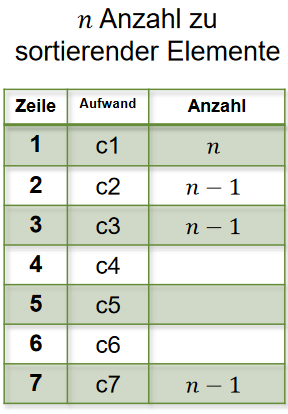
\includegraphics[width=0.25\textwidth]{Bilder/InsSortLZ.png}
                \caption{Beispiel von Insertion Sort}
                \label{fig:InsSortLZ}
            \end{figure}\\
            \begin{lstlisting}[style=pseudocode]
insertionSort(A)
    FOR i=1 TO A.length-1 DO //insert A[i] in pre-sorted sequence A[0..i-1]
        key=A[i];
        j=i-1; // search for insertion point backwards
        WHILE j>=0 AND A[j]>key DO
            A[j+1]=A[j]; // move elements to right
            j=j-1;
        A[j+1]=key;
            \end{lstlisting}
            Bei Insertion- Sort bedeutet das, dass Zeilen 4, 5 und 6 im schlimmsten Fall bis $j=-1$ also jeweils $i$-mal ausgeführt werden. Insgesamt: $\sum_{i=1}^{n-1}i=\frac{n(n-1)}{2}$ (Zeile 4 jeweils einmal mehr bis Abbruch)\\
            Maximale Gesamtlaufzeit Insertion-Sort: $T(n)=c2\cdot n+(c3+c4+c5+c8)\cdot (n-1)+(c5+c6+c7)\cdot \frac{n(n-1)}{2}$.
            Wie teuer ist z.B. Zuweisung $A[j+1]=A[j]$ in Zeile 5, also was ist $c6$? Hängt stark von Berechnungsmodell ab (in dem Pseudocode-Algorithmus umgesetzt wird)$\dots$. Wnehmen üblicherweise an, dass elementare Operationen (Zuweisung, Vergleich,…) in einem Schritt möglich $\rightarrow c6=1$.\\
            \begin{figure}[ht]
                \centering
                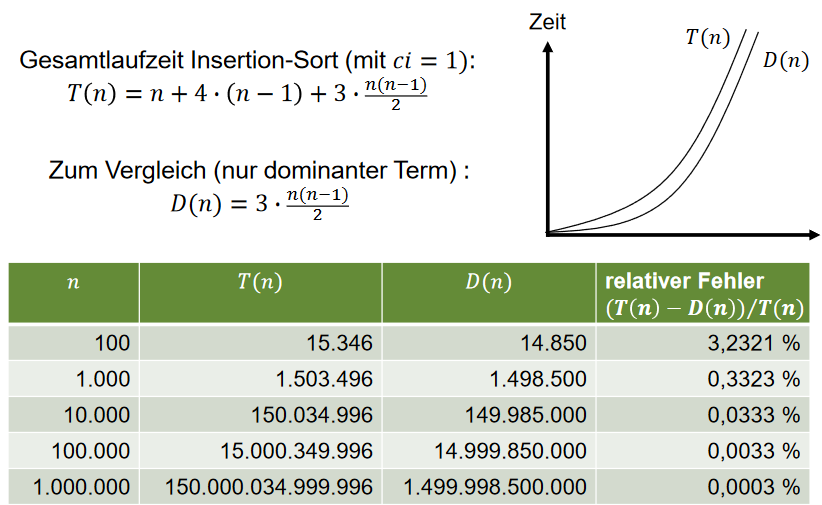
\includegraphics[width=0.75\textwidth]{Bilder/AsVer.png}
                \caption{Asymptotische Vereinfachung}
                \label{fig:AsVer}
            \end{figure}
            \newpage
            Weiter Vereinfachung (nur abhängiger Term): $A(n)=\frac{n(n-1)}{2}$.
            \subsubsection{$\Theta$- Notation}
                Auch Landau- Notation genannt.\\
                Wie nehmen eine Funktion $f,g: N \rightarrow R_{>0}$.\\
                \begin{figure}[ht]
                    \centering
                    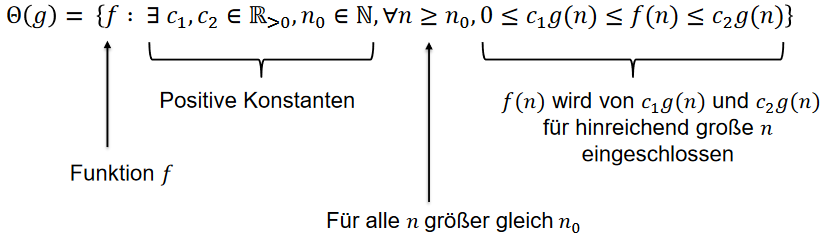
\includegraphics[width=0.75\textwidth]{Bilder/ThetaN.png}
                    \caption{Definition}
                    \label{fig:ThetaN}
                \end{figure}\\
                Schreibweise: $f\in \Theta(g)$, manchmal auch $f= \Theta(g)$.\\
                \begin{figure}[ht]
                    \centering
                    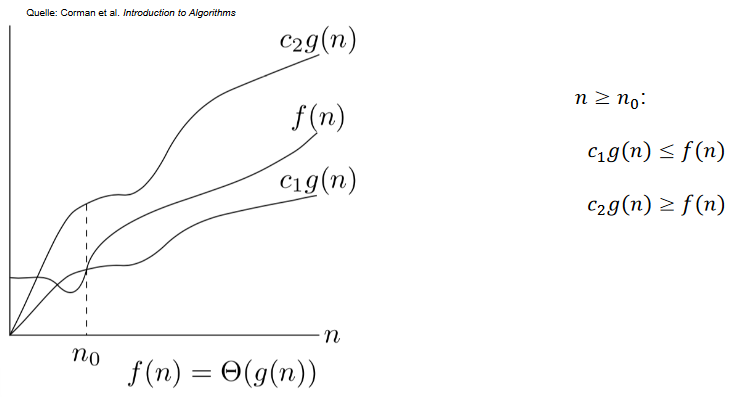
\includegraphics[width=0.75\textwidth]{Bilder/VeranschaulichungT.png}
                    \caption{Veranschaulichung $\Theta$-Notation}
                    \label{fig:VeranschaulichungTheta}
                \end{figure}\\
                \newpage
                $g(n)$ ist eine asymptotisch scharfe Schranke von $f(n)$. $\Theta$-Notation beschränkt eine Funktion asymptotisch von oben und unten.\\
                Bei Insertion Sort ergibt sich mit der oben angegebenen Formel $T(n)=n+4\cdot (n-1)+3\cdot \frac{n(n-1)}{2}=\Theta(n^2)$:
                \begin{itemize}
                    \item Untere Schranke ($c_1=\frac{3}{2}$): $\frac{3}{2}n^2$ für $n\geq 2$
                    \item Obere Schranke ($c_2=7$): $7\cdot n^2$
                \end{itemize} 
            \subsubsection{0- Notation}
                Auch als \textit{Obere Asymptotische Schranke} bezeichnet.\\
                \begin{figure}[ht]
                    \centering
                    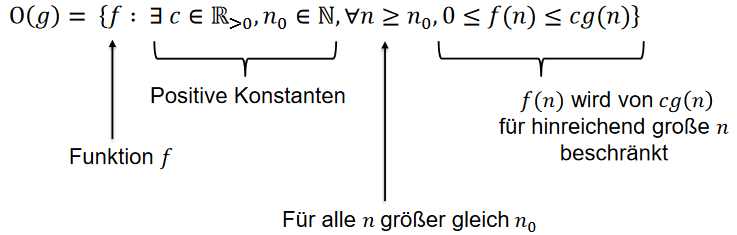
\includegraphics[width=0.75\textwidth]{Bilder/ON.png}
                    \caption{Definition}
                    \label{fig:ON}
                \end{figure}\\
                Sprechweise: $f$ wächst höchstens so schnell wie $g$.\\
                Schreibweise: $f=O(g)$ oder auch $f\in O(g)$.\\
                \begin{figure}[ht]
                    \centering
                    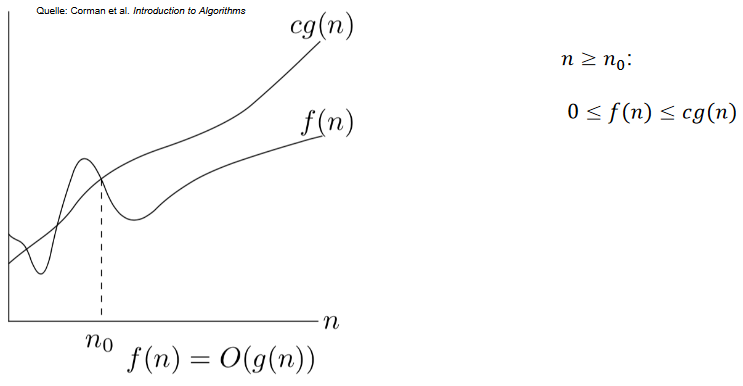
\includegraphics[width=0.75\textwidth]{Bilder/VeranschaulichungO.png}
                    \caption{Veranschaulichung O-Notation}
                    \label{fig:VeranschaulichungO}
                \end{figure}
                \newpage
                Beachte: $\Theta(g(n)) \subseteq O(g(n))$ und somit $f(n)=\Theta(g)\Rightarrow f(n)=O(g)$.\\
                Rechenregeln:
                \begin{itemize}
                    \item Konstanten: $f(n)=a$ mit $a\in R_{>0}$ konstant. Dann $f(n)=O(1)$
                    \item Skalare Multiplikation: $f=O(g)$ und $a\in R_{>0}$. Dann $a\cdot f=O(g)$
                    \item Addition: $f_1=O(g_1)$ und $f_2=O(g_2)$. Dann ist $f_1+f_2 =O(max\{g_1,g_2\})$
                    \item Multiplikation: $f_1=O(g_1)$ und $f_2=O(g_2)$. Dann $f_1\cdot f_2=O(g_1\cdot g_2)$
                \end{itemize}
            \subsubsection{$\Omega$- Notation}
                Auch als \textit{Untere Asymptotische Schranke} bezeichnet.\\
                \begin{figure}[ht]
                    \centering
                    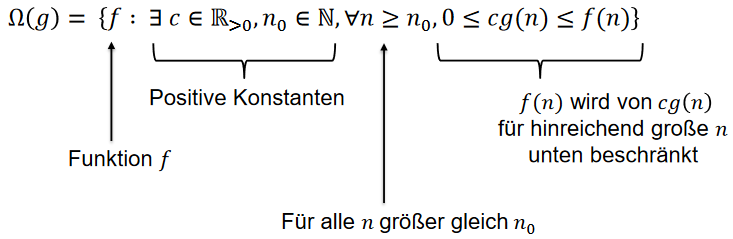
\includegraphics[width=0.75\textwidth]{Bilder/OmegaN.png}
                    \caption{Definition}
                    \label{fig:OmegaN}
                \end{figure}\\
                Sprechweise: $f$ wächst mindestens so schnell wie $g$.\\
                Schreibweise: $f=\Omega(g)$ oder auch $f\in \Omega(g)$.\\
                \begin{figure}[ht]
                    \centering
                    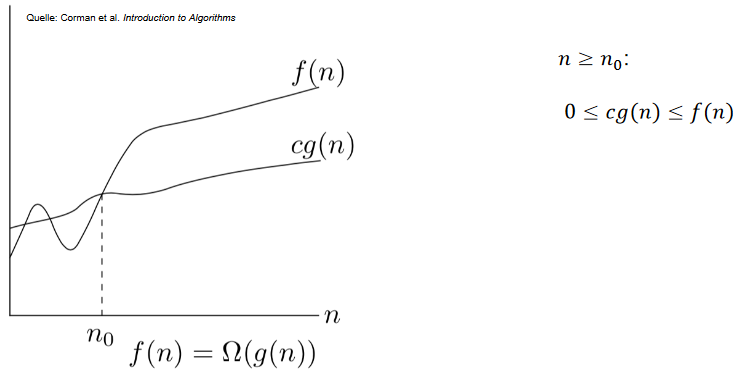
\includegraphics[width=0.75\textwidth]{Bilder/VeranschaulichungOmega.png}
                    \caption{Veranschaulichung $\Omega$-Notation}
                    \label{fig:VeranschaulichungOmega}
                \end{figure}\\
                \newpage
                Beachte: $\Theta(g(n)) \subseteq \Omega(g(n))$ und somit $f(n)=\Theta(g)\Rightarrow f(n)=\Omega(g)$.\\
            \subsubsection{Komplexitätsklassen}
                \begin{itemize}
                    \item $\Theta(1)$: Konstant (Bsp: Einzeloperation)
                    \item $\Theta(log n)$: Logarithmisch (Binäre Suche)
                    \item $\Theta(n)$: Linear (Sequentielle Suche)
                    \item $\Theta(n log n)$: Quasilinear (Sortieren eines Arrays)
                    \item $\Theta(n^2)$: Quadratisch (Matrixaddition)
                    \item $\Theta(n^3)$: Kubisch (Matrixmultiplikation)
                    \item $\Theta(n^k)$: Polynomiell
                    \item $\Theta(2^n)$: Exponentiell (Travelling-Salesman*)
                    \item $\Theta(n!)$: Faktoriell (Permutationen)
                \end{itemize}
            \subsubsection{o-Notation und $\omega$-Notation}
                $o(g)=\{f:\forall c\in R_{>0},\exists n_0\in N,\forall n \geq n_0,0\leq f(n)< cg(n)\}$ (Beispiel: $2n=o(n^2)$ und $2n^2\neq o(n^2)$).\\
                $\omega(g)=\{f:\forall c\in R_{>0},\exists n_0\in N,\forall n \geq n_0,0\leq cg(n)< f(n)\}$ (Beispiel: $\frac{n^2}{2}=\omega(n)$ und $\frac{n^2}{2} \neq \omega(n^2)$).\\

        \subsection{Merge- Sort}
            Auch \textit{Divide and Conquer- Algorithmus} genannt.\\
            \begin{figure}[ht]
                \centering
                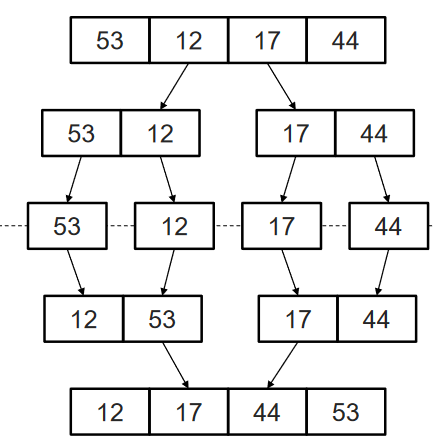
\includegraphics[width=0.35\textwidth]{Bilder/MergeSort.png}
                \caption{Visualisierung des Merge Sorts}
                \label{fig:mergesort}
            \end{figure}
            \newpage
            Teile Liste in Hälften, sortiere (rekursiv) Hälften, sortiere wieder zusammen.\\
            \begin{lstlisting}[style=pseudocode]
mergeSort(A,l,r) // initial call: l=0,r=A.length-1
    IF l<r THEN //more than one element
        m=floor((l+r)/2); // m (rounded down) middle (genauer: letzter Index des linken Teils)
        mergeSort(A,l,m); // sort left part
        mergeSort(A,m+1,r); // sort right part
        merge(A,l,m,r); // merge into one
            \end{lstlisting}
            Wir sortieren im Array A zwischen Position l (links) und r (rechts).\\
            \textbf{Merge:}\\
            Idee : nimm nächstes kleinstes Element aus linker oder rechter Teilliste und gehe in dieser Liste eine Position nach rechts.\\
            Jede Liste wird genau einmal durchlaufen $\Rightarrow$ Laufzeit $\Theta(n_L+n_R)$.\\
            \begin{lstlisting}[style=pseudocode]
merge(A,l,m,r) // requires l<=m<=r; array B with r-l+1 elements as temporary storage
    pl=l; pr=m+1; // position left, right
    FOR i=0 TO r-l DO // merge all elements
        IF pr>r OR (pl=<m AND A[pl]=<A[pr]) THEN
            B[i]=A[pl];
            pl=pl+1;
        ELSE //next element at pr
            B[i]=A[pr];
            pr=pr+1;
    FOR i=0 TO r-l DO A[i+l]=B[i]; //copy back to A
            \end{lstlisting}
            \begin{figure}[ht]
                \centering
                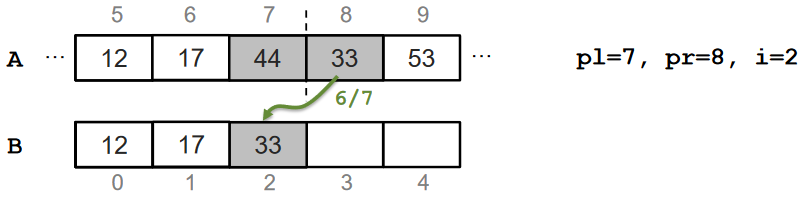
\includegraphics[width=0.75\textwidth]{Bilder/MergeBsp.png}
                \caption{Beispiel Merge, wenn er in einem Array dargestellt wird}
                \label{fig:MergeBsp}
            \end{figure}
            \begin{figure}[ht]
                \centering
                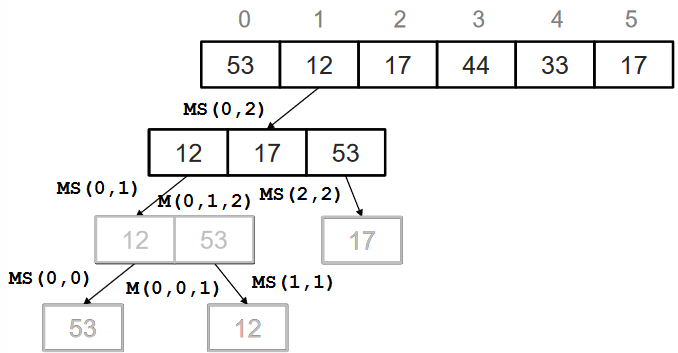
\includegraphics[width=0.75\textwidth]{Bilder/MergeSortBsp.png}
                \caption{Beispiel Merge- Sort aus der Mitte des Algorithmus}
                \label{fig:MergeSortBsp}
            \end{figure}
            \newpage
        \subsection{Mastertheorem}
            Seien $a \geq 1$ und $b > 1$ Konstanten. Sei $f(n)$ eine positive Funktion und $T(n)$ über den nicht-negativen ganzen Zahlen durch die Rekursionsgleichung $T(n)=aT(\frac{n}{b})++f(n)$, $T(1)=\Theta(1)$ definiert, wobei wir $\frac{n}{b}$ so interpretieren, dass damit entweder $\lceil n/b \rceil$ oder $\lfloor n/b \rfloor$gemeint ist. Dann besitzt $T(n)$ die folgenden asymptotischen Schranken:\\
            \begin{itemize}
                \item 1. Gilt $f(n)=O(n^{log_b (a)-\gamma})$ für eine Konstante $\gamma >0$, dann $T(n)=\Theta(n^{log_b a})$
                \item 2. Gilt $f(n)=\Theta(n^{log_b a})$, dann gilt $T(n)=\Theta(n^{log_b a}\cdot log_2 n)$
                \item 3. Gilt $f(n)=\Omega(n^{log_b (a)+\gamma})$ für eine Konstante $\gamma >0$ und $af(n/b) \leq cf(n)$ für eine Konstante $c<1$ und hinreichend große $n$, dann ist $T(n)=\Theta(f(n))$
            \end{itemize}
            \textbf{Interpretation} (entscheident ist Verhältnis von $f(n)$ zu $n^{log_b a}$)
            \begin{itemize}
                \item 1. Wenn $f(n)$ polynomiell kleiner als $n^{log_b a}$, dann $T(n)=\Theta(n^{log_b a})$
                \item 2. Wenn $f(n)$ und $n^{log_b a}$ gleiche Größenordnung, dann $T(n)=\Theta(n^{log_b a}\cdot log n)$
                \item 3. Wenn $f(n)$ polynomiell größer als $n^{log_b a}$ und $af(n/b)\leq cf(n)$, dann $T(n)=\Theta(f(n))$
            \end{itemize}
            'Regularität' $af(n/b)\leq cf(n)$, $c<1$ in Fall 3: $T(n)=a\cdot T(n/b)+f(n)=a\cdot (a\cdot T(n/b^2)+f(n/b))+f(n)$.\\
            \textit{Aufwand $f(n)$ zum Teilen und Zusammenfügen für Größe $n$ dominiert (asymptotisch) Summe $af(n/b)$ aller Aufwände für Größe $n/b$ braucht man nur im dritten Fall für 'große' $f(n)$}\\
            Der Unterschied zwischen 1 und 3 ist der polynomielle Faktor $n^\gamma$.\\
            \begin{figure}[ht]
                \centering
                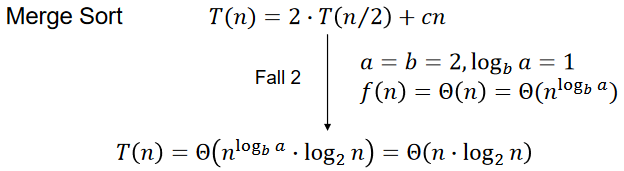
\includegraphics[width=0.75\textwidth]{Bilder/MTBsp.png}
                \caption{Beispiel Mastertheorem von Merge- Sort}
                \label{fig:MTBsp}
            \end{figure}
        \subsection{Quick- Sort}
            Wie in Merge- Sort verwendet Quicksort Divide and Conquer- Ansatz. \\
            Quicksort steckt mehr Arbeit in Aufteilen, Zusammenfügen kostenlos.\\
            \begin{figure}[ht]
                \centering
                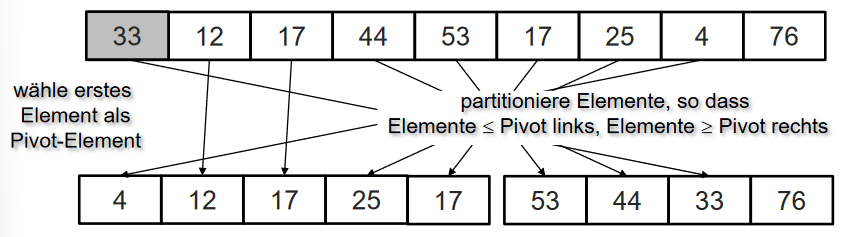
\includegraphics[width=0.75\textwidth]{Bilder/QuickSort.png}
                \caption{Erläuterung}
                \label{fig:QuickSort}
            \end{figure}\\
            Sortiert beide Teil-Arrays rekursiv, wobei das Ergebnis ein komplett sortiertes Array ist.\\
            \begin{lstlisting}[style=pseudocode]
quicksort(A,l,r) // initial call: l=0,r=A.length-1
    IF l<r THEN //more than one element
        p=partition(A,l,r); // p partition index
        quicksort(A,l,p); // sort left part
        quicksort(A,p+1,r); // sort right part
            \end{lstlisting}
            \begin{lstlisting}[style=pseudocode]
partition(A,l,r) //requires l<r, returns int in l..r-1
    pivot=A[l];
    pl=l-1; pr=r+1; //move from left resp. right
    WHILE pl<pr DO
        REPEAT pl=pl+1 UNTIL A[pl]>=pivot; //move left up
        REPEAT pr=pr-1 UNTIL A[pr]=<pivot; //move right down
        IF pl<pr THEN Swap(A[pl],A[pr]);
        p=pr; //store current value
    RETURN p // A[l..p] left, A[p+1..r] right
            \end{lstlisting}
            Hier ein Beispiel von Partition, mit \textit{pivot=12, l=2, r=6}:\\
            \begin{figure}[ht]
                \centering
                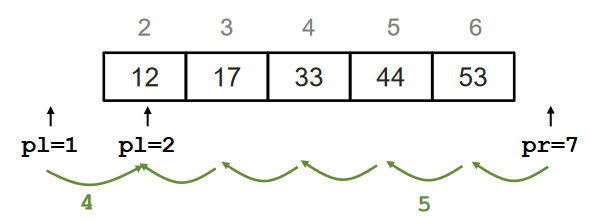
\includegraphics[width=0.5\textwidth]{Bilder/Partition1.png}
                \caption{Beispiel der Suche nach den zu tauschenden Elementen}
                \label{fig:Partition1}
            \end{figure}\\
            Daraus folgt P\textit{p=2}.\\
            \begin{figure}[ht]
                \centering
                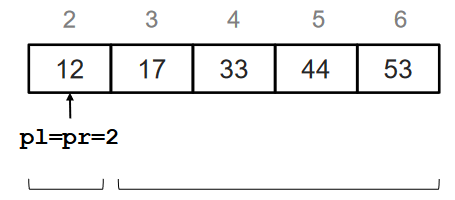
\includegraphics[width=0.5\textwidth]{Bilder/Partition2.png}
                \caption{Beispiel bei der Findung des Elements}
                \label{fig:Partition2}
            \end{figure}\\
            In diesem Fall haben wir jedoch pl=pr, deswegen kein Swap.\\
            Ein Beispiel- Swap wäre:
            \begin{figure}[ht]
                \centering
                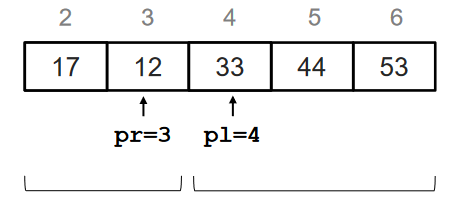
\includegraphics[width=0.5\textwidth]{Bilder/Partition3.png}
                \caption{ }
                \label{fig:Partition3}
            \end{figure}\\
            Daraufhin werden 12 und 17 geswaped (mit \textit{pivot=33, p=3}).\\
            \textbf{Laufzeit} Partition:\\
            Für jede Erhöhung von pl bzw. Erniedrigung von pr konstant viele Schritte:
            \begin{itemize}
                \item \textit{pl} und \textit{pr} haben zu Beginn Abstand $n+2$ und bewegen sich in jeder Iteration aufeinander zu $\Rightarrow O(n)$
                \item \textit{pl} und \textit{pr} bewegen sich in jeder einzelnen REPEAT-Iteration maximal 1 aufeinander zu $\Rightarrow \Omega(n)$
            \end{itemize}
            Laufzeit Partition: $\Theta(n)$.
            \subsubsection{Laufzeitanalyse QuickSort}
                \textbf{Worst-Case}:
                \begin{itemize}
                    \item \textbf{Untere Schranke:} Ungünstiges Array: Partition spaltet immer nur ein Element ab. $(n-1)$-mal Partition ergibt Quicksort Gesamtlaufzeit$\Omega(n^2)$.
                    \item \textbf{Obere Schranke:} $T(n)\leq dn^2$
                \end{itemize}
                Quicksort (Worst-Case-)Laufzeit: $\Theta(n^2)$\\
                \textbf{Best- Case}:
                \begin{itemize}
                    \item Im besten Fall Aufteilung in gleichgroße Arrays wie bei Merge Sort: $T(n)=2T(n+2)+\Theta(n) \Rightarrow$ Laufzeit $\Theta(n\cdot log n)$
                \item Gilt auch, solange beide Arrays in Größenordnung $\Omega(n)$, z.B. stets 10\% der $n$ Elemente links und 90\% rechts: $T(n)=T(0.1n)+T(0.9n)+\Theta(n)$ Laufzeit $\Theta(n\cdot log n)$
                \end{itemize}
                \textbf{Average}:\\
                Wie verhält sich Quicksort im Durchschnitt auf 'zufälliger' Eingabe?\\
                Für zufällige Permutation $D(n)$ eines fixen Arrays von $n$ Elementen benötigt Quicksort $E_{D(n)}[Anzahl Schritte]=O(n\cdot log n)$
            \begin{figure}[ht]
                \centering
                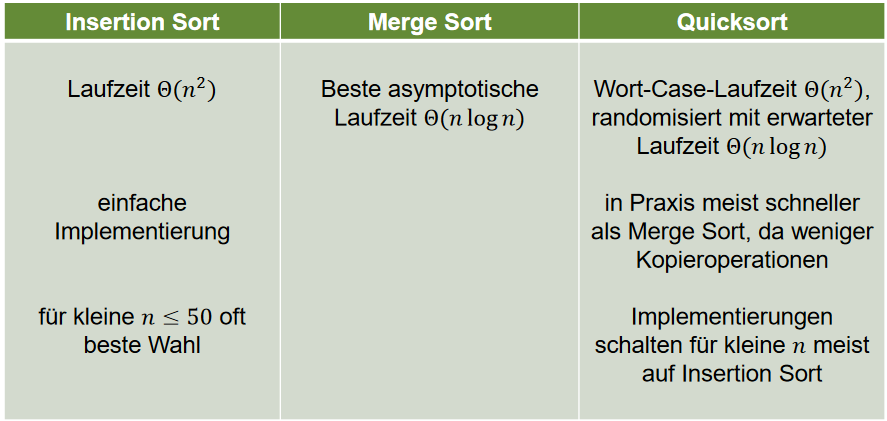
\includegraphics[width=0.75\textwidth]{Bilder/VerglInMeundQu.png}
                \caption{Vergleich: Insertion, Merge, und Quicksort}
                \label{fig:VerglInMeundQu}
            \end{figure}
        \subsection{Radix- Sort}
            Ansatz: Schlüssel sind d-stellige Werte in D-närem Zahlensystem:\\
            \begin{figure}[ht]
                \centering
                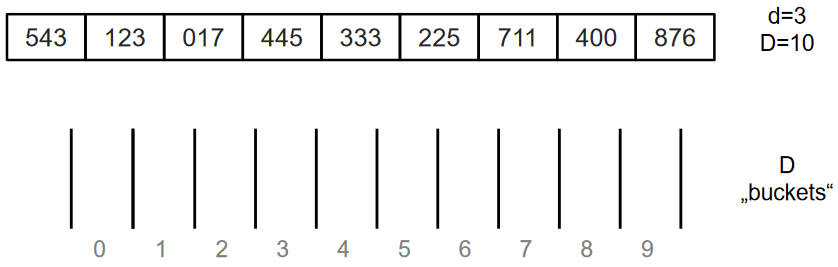
\includegraphics[width=0.75\textwidth]{Bilder/RadixBsp.png}
                \caption{Beispiel}
                \label{fig:RadixBsp}
            \end{figure}\\
            'Buckets' erlauben Einfügen und dann Entnehmen (in eingefügter Reihenfolge) in konstanter Zeit.\\
            Dabei gehen wir alle Zahlen von der kleinstwertigen zur größtwertigsten Stelle durch und fügen diese in die Buckets ein, danach verschieben wir diese wieder in den Array.
            \begin{figure}[ht]
                \centering
                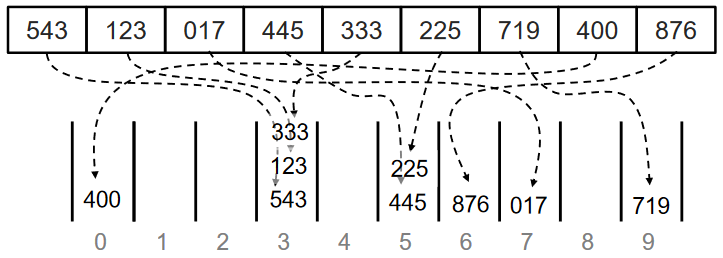
\includegraphics[width=0.75\textwidth]{Bilder/Radix1.png}
                \caption{Erste Iteration des Beispiels, also kleinstwertige Stelle}
                \label{fig:Radix1}
            \end{figure}\\
            \begin{figure}[ht]
                \centering
                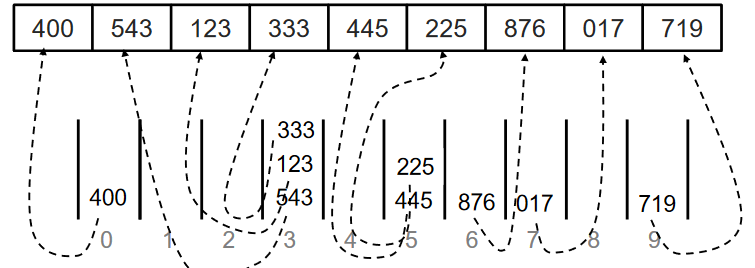
\includegraphics[width=0.75\textwidth]{Bilder/Radix2.png}
                \caption{Einfügen nach dem aufteilen in die Buckets}
                \label{fig:Radix2}
            \end{figure}\\
            Nachdem wir dies für jede Ziffer machen, haben wir eine sortierte Liste.\\
            \begin{lstlisting}[style=pseudocode]
radixSort(A) // keys: d digits in range [0,D-1]; B[0][],..., B[D-1][] buckets (init: B[k].size=0)
    FOR i=0 TO d-1 DO //0 least, d-1 most sign. digit
        FOR j=0 TO n-1 DO putBucket(A,B,i,j);
        a=0;
        FOR k=0 TO D-1 DO //rewrite to array
            FOR b=0 TO B[k].size-1 DO
                A[a]=B[k][b]; //read out bucket in order
                a=a+1;
            B[k].size=0; //clear bucket again
    RETURN A;
            \end{lstlisting}
            \textbf{Laufzeit:} $O(d\cdot (n+D))$.
            \begin{lstlisting}[style=pseudocode]
putBucket(A,B,i,j) // call-by-reference
    z=A[j].digit[i]; // i-th digit of A[j]
    b=B[z].size; // next free spot
    B[z][b]=A[j];
    B[z].size=B[z].size+1;
            \end{lstlisting}
            \textbf{laufzeit:} $O(1)$.\\
            \begin{figure}[ht]
                \centering
                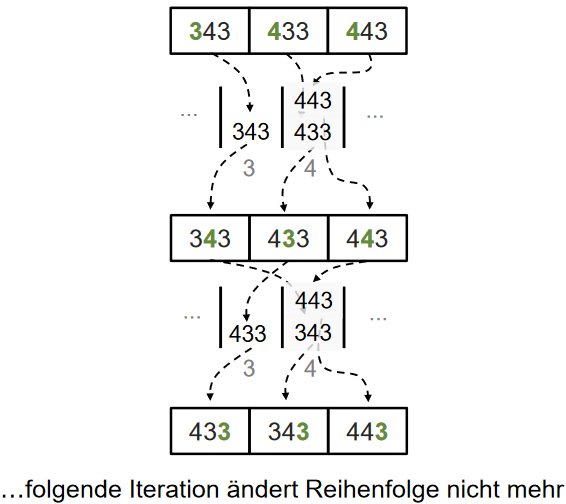
\includegraphics[width=0.75\textwidth]{Bilder/RadixW.png}
                \caption{Warum man nicht mit der größtwertigsten Ziffer beginnen kann}
                \label{fig:RadixW}
            \end{figure}\\

    \newpage

    \section{Basic Data Strctures}
        \subsection{Stacks}
            Als Stacks bezeichnet man eine abstrakte Datenstruktur, die mit den LIFO- Prinzip arbeitet (Last in, First out). 
            \begin{figure}[ht]
                \centering
                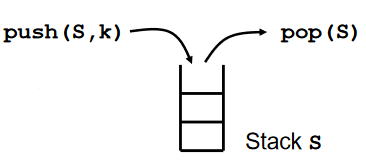
\includegraphics[width=0.5\textwidth]{Bilder/LIFOStacks.png}
                \caption{Visualisierung von LIFO eines Stacks S}
                \label{fig:LIFO}
            \end{figure}
            Dabei haben Stacks folgende Operationen: 
            \begin{itemize}
                \item new(S) - erzeugt neuen (leeren) Stack namens S
                \item isEmpty(S) - gibt an, ob Stack S leer
                \item pop(S) - gibt oberstes Element vom Stack S zurück und löscht es vom Stack (bzw. Fehlermeldung, wenn Stack leer)
                \item push(S,k) - schreibt k als neues oberstes Element auf Stack S (bzw. Fehlermeldung, wenn Stack voll)
            \end{itemize}
            Man kann einen Stack auch als Array darstellen. Dabei wird das Element im Array, welches den größten Index hat, als Top gesehen. \\
            Wenn man den Stack als Array darstellt, ergeben sich folgende Methoden:
            \begin{lstlisting}[style=pseudocode]
new(S)
    S.A[]=ALLOCATE(MAX);
    S.top=-1;
            \end{lstlisting}
            \begin{lstlisting}[style=pseudocode]
isEmpty(S)
    IF S.top<0 THEN
        RETURN true;
    ELSE
        RETURN false;
            \end{lstlisting}
            \begin{lstlisting}[style=pseudocode]
pop(S)
    IF isEmpty(S) THEN
        error "underflow";
    ELSE
        S.top=S.top-1;
        RETURN S.A[S.top+1];
            \end{lstlisting}
            Laufzeit: $\Theta(1)$
            \begin{lstlisting}[style=pseudocode]
push(S,k)
    IF S.top==MAX-1 THEN
        error "overflow";
    ELSE
        S.top=S.top+1;
        S.A[S.top]=k;
            \end{lstlisting}
            Laufzeit: $\Theta(1)$\\
            Man kann auch Stacks mit Variabler Größe machen, bei der bei vollem Stack immer ein neuer Stack erstellt wird (Effizient: Größe x2) und alle bisherige Einträge kopiert werden.\\
            \textbf{Laufzeitanalyse}, gilt für Vergrößerung und Verkleinerung:\\
            (1) $n$ Elemente (unmittelbar nach letzter Vergrößerung) \\
            (2) neue Speichergrenze wird nur erreicht, wenn dann mindestens $n$ viele Push-Befehle \\
            (3) Umkopieren kostet dann $O(n)$ Schritte \\
            Im Durchschnitt für jeden der mindestens $n$ Befehle $\Theta(n)$ Umkopierschritte!
        \subsection{Verkettete Listen}
            Eine verkettete Liste ist eine Datenstruktur, bei der das Element immer zusätzlich auf den Vorgänger und den Nachfolger verweist.
            \begin{itemize}
                \item key: Wert
                \item prev: Zeiger auf Vorgänger (oder $nil$)
                \item next: Zeiger auf Nachfolger (oder $nil$)
            \end{itemize}
            Zusätzlich noch head (Zeigt auf das erste Element ($nil$ bei leerer Liste)).\\
            Des weiteren gibt es noch folgende Elementare Operationen:
            \begin{lstlisting}[style=pseudocode]
search(L,k) //RETURNs pointer to k in L (or nil)
    current=L.head;
    WHILE current != nil AND current.key != k DO
        current=current.next;
    RETURN current;
            \end{lstlisting}
            Laufzeit: $\Theta(n)$
            \begin{lstlisting}[style=pseudocode]
insert(L,x) //inserts element x in L
    x.next=L.head;
    x.prev=nil;
    IF L.head != nil THEN
        head.prev=x;
    L.head=x;
            \end{lstlisting}
            Laufzeit: $\Theta(1)$\\
            Hierbei wird nicht überprüft, ob das Element vorhanden ist. Wenn man vorher noch sucht, dann hat man Laufzeit $\Omega(n)$.
            \begin{lstlisting}[style=pseudocode]
delete(L,x) //deletes element x from L
    IF x.prev != nil THEN
        x.prev.next=x.next
    ELSE
        L.head=x.next;
    IF x.next != nil THEN
        x.next.prev=x.prev;
            \end{lstlisting}
            Laufzeit: $\Theta(1)$\\
            Es gibt auch noch einen Sentinel, welcher ein nicht sichtbarer Knoten ist, für den gilt (L ist die Liste):
            \begin{itemize}
                \item L.sent = head.prev
                \item head = L.sent.next
                \item Leere Liste besteht nur aus Sentinel
            \end{itemize}
            Eine angepasste Operation wäre:
            \begin{lstlisting}[style=pseudocode]
deleteSent(L,x) // deletes x from L with sentinel
    x.prev.next=x.next;
    x.next.prev=x.prev;
            \end{lstlisting}
            Andere Operationen müssen auch angepasst werden.
        \subsection{Queues}
            Als Queue bezeichnet man eine abstrakte Datenstruktur, die mit den FIFO- Prinzip arbeitet (First in, First out). 
            \begin{figure}[ht]
                \centering
                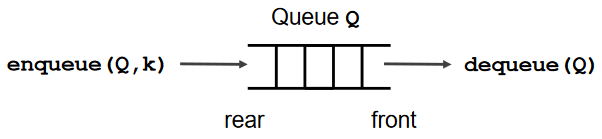
\includegraphics[width=0.6\textwidth]{Bilder/QueueFIFO.png}
                \caption{Visualisierung von FIFO einer Queue Q}
                \label{fig:FIFO}
            \end{figure}
            Dabei hat eine Queue folgende Operationen:
            \begin{itemize}
                \item new(Q) - erzeugt neue (leere) Queue namens Q
                \item isEmpty(Q) - gibt an, ob Queue Q leer
                \item dequeue(Q) - gibt vorderstes Element der Queue Q zurück und löscht es aus Queue (bzw. Fehlermeldung, wenn Queue leer)
                \item enqueue(Q,k) - schreibt k als neues hinterstes Element auf Q (bzw. Fehlermeldung, wenn Queue voll)
            \end{itemize}
            Man kann auch Queues als Array darstellen, jedoch ist dies schwierig. Denn entweder ist der Array irgendwann voll, oder es wird Speicherplatz verschwendet.\\
            Eine Lösung ist ein zyklischer Array:
            \begin{figure}[ht]
                \centering
                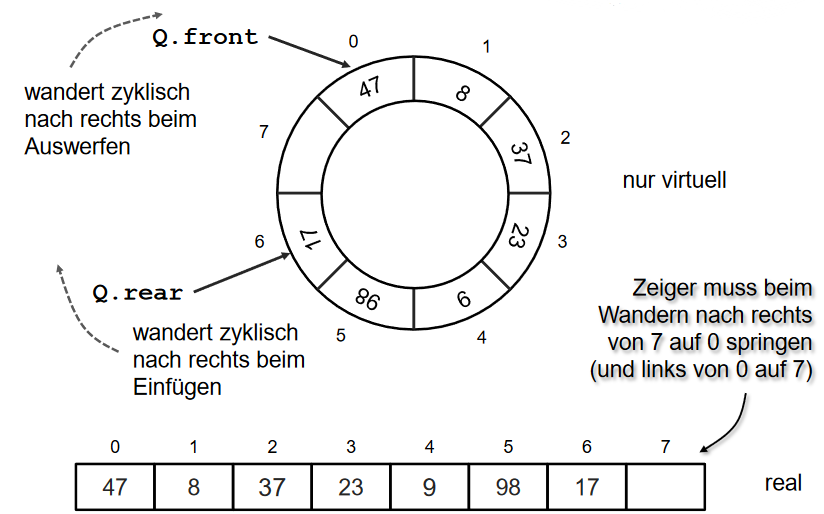
\includegraphics[width=1\textwidth]{Bilder/ZyklischerArray.png}
                \caption{Queues als (virtuelles) zyklisches Array}
                \label{fig:ZyklischerArray}
            \end{figure}
            Um zu Wissen, ob die zyklische Queue voll oder leer ist, muss man dies in einer Variable speichern, oder alternativ ein Element des Arrays als Abstandhalter reservieren.
            Algorithmen bei Queues als zyklischer Array: \\
            \textit{Hierbei gilt: Q leer, wenn front == rear und empty == true und voll, wenn front == rear und empty = false}\\
            \begin{lstlisting}[style=pseudocode]
new(Q)
    Q.A[]=ALLOCATE(MAX);
    Q.front=0;
    Q.rear=0;
    Q.empty=true;
            \end{lstlisting}
            \begin{lstlisting}[style=pseudocode]
isEmpty(Q)
    RETURN Q.empty;
            \end{lstlisting}
            \begin{lstlisting}[style=pseudocode]
dequeue(Q)
    IF isEmpty(Q) THEN
        error "underflow";
    ELSE
        Q.front=Q.front+1 mod MAX;
        IF Q.front==Q.rear THEN
            Q.empty=true;
        RETURN Q.A[Q.front-1 mod MAX];
            \end{lstlisting}
            Laufzeit: $\Theta(1)$
            \begin{lstlisting}[style=pseudocode]
enqueue(Q,k)
IF Q.rear==Q.front AND !Q.empty
    error "overflow";
ELSE
    Q.A[Q.rear]=k;
    Q.rear=Q.rear+1 mod MAX;
    Q.empty=false;
            \end{lstlisting}
            Laufzeit: $\Theta(1)$\\
            Man kann eine Queue auch durch eine einfache! verkettete Liste darstellen, wessen Algorithmen aber leichter sind.
        \subsection{Binärer Baum}
            \begin{figure}[ht]
                \centering
                \includegraphics[width=0.75\textwidth]{Bilder/BinärerBaum.png}
                \caption{Darstellung eines binären Baums}
                \label{fig:BinaererBaum}
            \end{figure}
            Das ist ein binärer Baum.\\
            Jeder Knoten enthält:
            \begin{itemize}
                \item key - Wert
                \item child[] - Array von Zeigern auf Kinder
                \item parent - Zeiger auf Elterknoten (oder bei root $nil$)
            \end{itemize}
            \textbf{Baum-Bedingungen:} Baum ist leer oder es gibt einen Knoten r (Wurzel), so dass jeder Knoten v von der Wurzel aus per eindeutiger Sequenz von child-Zeigern erreichbar ist: v = r.child[i1].child[i2].….child[im]. \\
            Außerdem sind Bäume azyklisch (Man kann keinen Zyklus bilden). \\
            Man kann Binäre Bäume auch als ungerichtete Graphen darstellen, welches wir ab jetzt tun werden.\\
            \textbf{Begrifflichkeiten:}
            \begin{figure}[ht]
                \centering
                \includegraphics[width=0.75\textwidth]{Bilder/BinärerBaumBegrifflichkeiten.png}
                \label{fig:BinaererBaumBegrifflichkeiten}
            \end{figure}\\
            Außerdem gilt:
            \begin{itemize}
                \item Jeder Knoten hat maximal zwei Kinder: left=child[0] und0 right=child[1]
                \item Ein "Halbblatt" hat genau ein Kinder
                \item Ein Knoten $z$ hat einen linken und rechten Teilbaum, falls left und right != nil
                \item Als Teilbaum bezeichnet man alle Knoten, die sich auf dieser Seite des Knotens befinden (Bsp: child[0], child[0].child[0], child[0].child[1]...)
                \item Höhe (Nicht leerer) Baum = $max${Höhe aller Teilbäume der Wurzel }$ +1$
                \item Höhe leerer Baum hier per Konvention -1
            \end{itemize}

            \textbf{Traversierungen von Binärbäumen:}\\
            \textit{Nehmen wir für die Beispiele die Abbildung der Begrifflichkeiten.}\\
            Inorder- Traviersierung:
            \begin{lstlisting}[style=pseudocode]
inorder(x)
    IF x != nil THEN
        inorder(x.left);
        print x.key;
        inorder(x.right);
            \end{lstlisting} 
            Beispiel: inorder(T.root) = [23 , 9 , 17 , 5 , 12 , 23] \\
            Wichtig ist noch: Verschiedene Bäume können gleiche Inorder haben. \\
            Preorder- Traviersierung:
            \begin{lstlisting}[style=pseudocode]
preorder(x)
    IF x != nil THEN
        print x.key;
        preorder(x.left)
        preorder(x.right);
            \end{lstlisting} 
            Beispiel: preorder(T.root) = [5 , 9 , 23 , 17 , 12 , 23] \\
            Wichtig ist noch: Verschiedene Bäume können gleiche Preorder haben. \\
            Postorder- Traviersierung:
            \begin{lstlisting}[style=pseudocode]
postorder(x)
    IF x != nil THEN
        postorder(x.left)
        postorder(x.right);
        print x.key;
            \end{lstlisting} 
            Beispiel: postorder(T.root) = [23 , 17 , 9 , 23 , 12 , 5] \\
            Dabei ergeben jedoch Preorder + Inorder + eindeutige Werte einen Binärbaum: \\
            \begin{figure}[ht]
                \centering
                \includegraphics[width=0.75\textwidth]{Bilder/OrderBinärBaum.png}
                \caption{Beispiel}
                \label{fig:OrderBinär}
            \end{figure}\\
            \subsubsection{Abstrakter Datentyp- Baum}
                Operationen:
                \begin{lstlisting}[style=pseudocode]
search(x,k)
    IF x==nil
        RETURN nil;
    IF x.key==k
        RETURN x;
    y=search(x.left,k);
    IF y != nil
        RETURN y;
    RETURN search(x.right,k);
                \end{lstlisting}
                Dabei startet man mit search(T.root, k); \textbf{Laufzeit:} $\Theta(n)$
                \begin{lstlisting}[style=pseudocode]
insert(T,x)
    IF T.root != nil THEN
        T.root.parent=x;
        x.left=T.root;
    T.root=x;
                \end{lstlisting}
                \textbf{Laufzeit:} $\Theta(1)$\\
                Wenn der eingefüge Knoten die neue Wurzel ist, ensteht ein einsietiger Baum.\\
                \begin{lstlisting}[style=pseudocode]
delete(T,x) //assumes x in T
    y=T.root;
    WHILE y.right!=nil DO
        y=y.right;
    connect(T,y,y.left);
    IF x != y THEN
        y.left=x.left;
        IF x.left != nil THEN
            x.left.parent=y;
        y.right=x.right;
        IF x.right != nil THEN
            x.right.parent=y;
    connect(T,x,y);
                \end{lstlisting}
                Beim löschen muss man beachten, dass wenn ein Halbblatt gelöscht wird, der Knoten durch das Halbblatt ganz rechts ersetzt wird, aber es geht auch ander:
                \begin{figure}[ht]
                    \centering
                    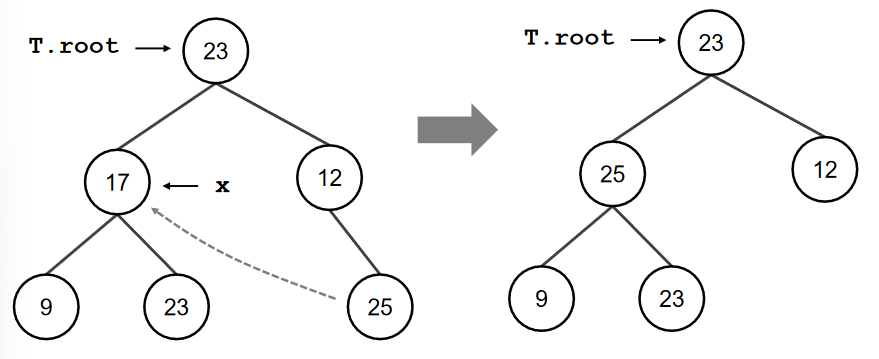
\includegraphics[width=0.75\textwidth]{Bilder/HalbblattBaum.png}
                    \caption{Visualisierung}
                    \label{fig:HalbblattBaum}
                \end{figure}\\
                \textbf{Laufzeit:} $\Theta(h)$
                Allgemein ist das Löschen aber je nach Knoten sehr individuell. 
        \subsection{Binärer Suchbaum (BST)}
            Ein binärer Suchbaum ist ein Binärer Baum, bei dem wir wieder totale Ordnung annehmen. \\
            Im Binären Suchbaum gilt für jeden Knoten $z$: 
            \begin{itemize}
                \item Wenn $x$ Knoten im linken Teilbaum von $z$, dann $x.key <= z.key$
                \item Wenn $y$ Knoten im rechten Teilbaum von $z$, dann $y.key >= z.key$
            \end{itemize}
            Beispiel:
            \begin{center}
            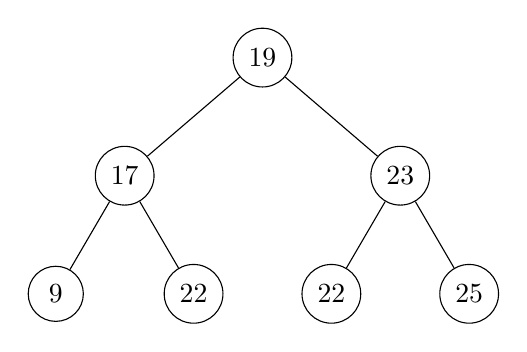
\begin{tikzpicture}[
                every node/.style={circle, draw, minimum size=0.7cm},
                level/.style={sibling distance=3.5cm/#1},
                level 2/.style={level distance=1.5cm},
              ]
              \node {19}
                child {node {17}
                  child {node {9}}
                  child {node {22}}
                }
                child {node {23}
                child {node {22}}
                  child {node {25}}
                };
              \end{tikzpicture}
              \end{center}
            Zumal gilt: 
            \begin{itemize}
                \item preorder + eindeutige Werte $=$ Binärer Suchbaum
                \item inorder + eindeutige Werte $\neq$ Binärer Suchbaum
            \end{itemize}
            \begin{lstlisting}[style=pseudocode]
search(x,k) //1.Aufruf x=root
    IF x==nil OR x.key==k THEN
        RETURN x;
    IF x.key > k THEN
        RETURN search(x.left,k)
    ELSE
        RETURN search(x.right,k);
            \end{lstlisting}
            \textbf{Laufzeit:} $O(h)$, h 0 Höhe des Baumes
            \begin{lstlisting}[style=pseudocode]
iterative-search(x,k) //Aufruf x=root
    WHILE x != nil AND x.key != k DO
        IF x.key > k THEN
            x=x.left
        ELSE
            x=x.right;
    RETURN x;
            \end{lstlisting}
            \begin{lstlisting}[style=pseudocode]
insert(T,z) //may insert z again z.left==z.right==nil;
    x=T.root; px=nil;
    WHILE x != nil DO
        px=x;
        IF x.key > z.key THEN
            x=x.left
        ELSE
            x=x.right;
    z.parent=px;
    IF px==nil THEN
        T.root=z
    ELSE
        IF px.key > z.key THEN
            px.left=z
        ELSE
            px.right=z;
            \end{lstlisting}
            \textbf{Laufzeit:} $O(h)$

            \vspace{30pt}
            \textbf{Löschen:}
            \begin{lstlisting}[style=pseudocode]
delete(T,z)
    IF z.left==nil THEN
        transplant(T,z,z.right)
    ELSE
        IF z.right==nil THEN
            transplant(T,z,z.left)
        ELSE
            y=z.right;
            WHILE y.left != nil DO y=y.left;
            IF y.parent != z THEN
                transplant(T,y,y.right);
                y.right=z.right;
                y.right.parent=y;
            transplant(T,z,y);
            y.left=z.left;
            y.left.parent=y;
            \end{lstlisting}
            \textbf{Laufzeit:} $O(h)$, h ist die Höhe des Baumes
            \begin{lstlisting}[style=pseudocode]
transplant(T,u,v)
    IF u.parent==nil THEN
        T.root=v
    ELSE
        IF u==u.parent.left THEN
            u.parent.left=v
        ELSE
            u.parent.right=v;
    IF v != nil THEN
        v.parent=u.parent;
            \end{lstlisting}
            \textbf{Laufzeit:} $\Theta(1)$\\
            Zu löschender Knoten z hat maximal ein Kind: \\
            \begin{figure}[ht]
                \centering
                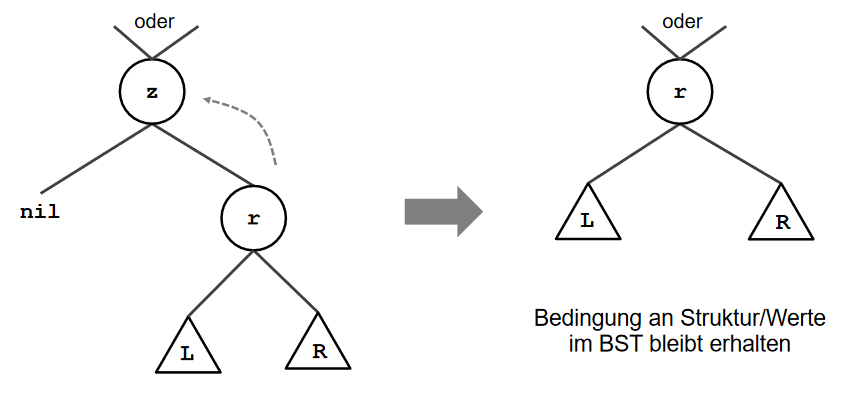
\includegraphics[width=0.75\textwidth]{Bilder/BSTdel1.png}
                \caption{Visualisierung}
                \label{fig:BSTdel1}
            \end{figure}\\
            Rechtes Kind von Knoten z hat kein linkes Kind: \\
            \begin{figure}[ht]
                \centering
                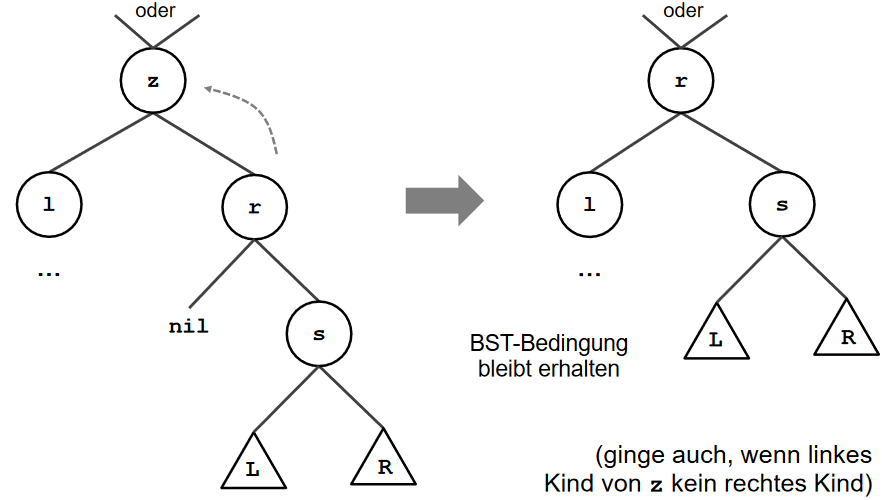
\includegraphics[width=0.75\textwidth]{Bilder/BSTdel2.png}
                \caption{Visualisierung}
                \label{fig:BSTdel2}
            \end{figure}\\
            'Kleinster' Nachfahre vom rechten Kind von z: \\
            \begin{figure}[ht]
                \centering
                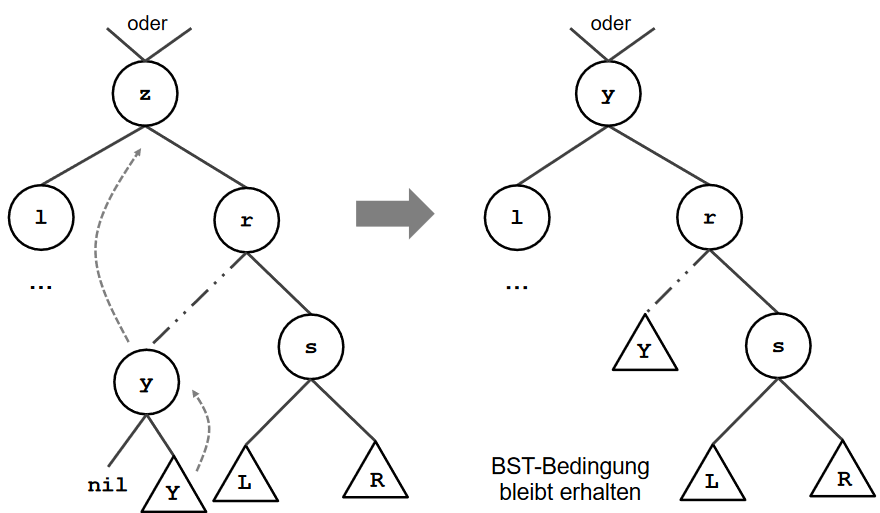
\includegraphics[width=0.75\textwidth]{Bilder/BSTdel3.png}
                \caption{Visualisierung}
                \label{fig:BSTdel3}
            \end{figure}\\
            \newpage
            Die Laufzeiten sind hierbei abhängig von der Höhe des BST. \\
            Die Best- Case Laufzeit ist $O(log_2n)$, wenn der BSt vollständig ist (alle Blätter haben gleiche Tiefe).\\
            Die Worst-Case Laufzeit ist $\Omega(n)$, wenn der BST degeneriert ist (Baum besteht aus einer linearen Liste).\\

    \newpage
    \section{Advanced Data Structures}
        \subsection{Rot- Schwarz- Bäume}
            Ein Rot-Schwarz-Baum ist ein binärer Suchbaum, so dass gilt:
            \begin{itemize}
                \item Jeder Knoten hat die Farbe rot oder schwarz
                \item Die Wurzel ist schwarz (sofern Baum nicht leer)
                \item Wenn ein Knoten rot ist, sind seine Kinder schwarz (Nicht- Rot- Rot- Regel)
                \item Für jeden Knoten hat jeder Pfad im Teilbaum zu einem Blatt oder Halbblatt die gleiche Anzahl von schwarzen Knoten (gleiche Anzahl schwarz)
                \item Hälbblätter sind schwarz
            \end{itemize}
            Dabei hat jeder Knoten noch einen besonderen Eintrag (x.color = red / black)\\
            \textbf{Beispiel:} \\
            \begin{figure}[ht]
                \centering
                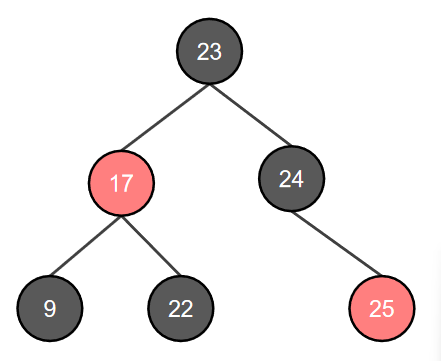
\includegraphics[width=0.5\textwidth]{Bilder/RSB.png}
                \caption{Ein Rot- Schwarz- Baum}
                \label{fig:RSB}
            \end{figure}\\
            Die Schwarzhöhe eines Knoten x ist die (eindeutige) Anzahl von schwarzen Knoten auf dem Weg zu einem Blatt oder Halbblatt im Teilbaum des Knoten. Außerdem muss die Schwarzhöhe am Knoten für jeden Pfad gleich sein.\\

            \textbf{Einfügen:}\\
            Rotation: \\
            \begin{figure}[ht]
                \centering
                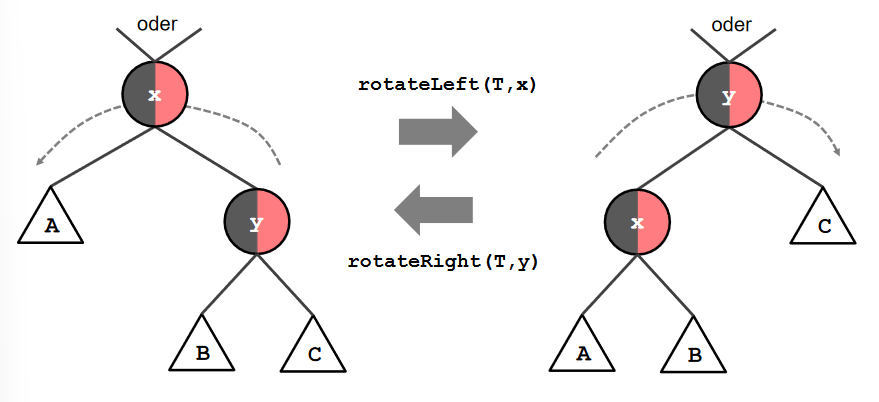
\includegraphics[width=0.75\textwidth]{Bilder/RSRotation.png}
                \caption{Rotation}
                \label{fig:RSRotation}
            \end{figure}\\
            \newpage
            \begin{lstlisting}[style=pseudocode]
rotateLeft(T,x) //x.right!=nil
    y=x.right;
    x.right=y.left;
    IF y.left != nil THEN
        y.left.parent=x;
    y.parent=x.parent;
    IF x.parent==T.sent THEN
        T.root=y
    ELSE
        IF x==x.parent.left THEN
            x.parent.left=y
        ELSE
            x.parent.right=y;
    y.left=x;
    x.parent=y;
            \end{lstlisting}
            \textbf{Laufzeit:} $\Theta(1)$.
            \begin{lstlisting}[style=pseudocode]
insert(T,z) //z.left==z.right==nil;
    x=T.root; px=T.sent;
    WHILE x != nil DO
        px=x;
        IF x.key > z.key THEN
            x=x.left
        ELSE
            x=x.right;
    z.parent=px;
    IF px==T.sent THEN
        T.root=z
    ELSE
        IF px.key > z.key THEN
            px.left=z
        ELSE
            px.right=z;
    z.color=red;
    fixColorsAfterInsertion(T,z);
            \end{lstlisting}
            \begin{lstlisting}[style=pseudocode]
fixColorsAfterInsertion(T,z)
    WHILE z.parent.color==red DO
        IF z.parent==z.parent.parent.left THEN
            y=z.parent.parent.right;
            IF y!=nil AND y.color==red THEN
                z.parent.color=black;
                y.color=black;
                z.parent.parent.color=red;
                z=z.parent.parent;
            ELSE
                IF z==z.parent.right THEN
                    z=z.parent;
                    rotateLeft(T,z);
                z.parent.color=black;
                z.parent.parent.color=red;
                rotateRight(T,z.parent.parent);
        ELSE
            ... //exchange left and right
    T.root.color=black;
            \end{lstlisting}
            \textbf{Laufzeit:} $O(n)=O(log_n)$\\
            \textbf{Schleifeninvariante:}
            \begin{itemize}
                \item z.color==red
                \item Wenn z.parent Wurzel, dann z.parent.color==black
                \item Wenn der aktuelle Baum kein Rot-Schwarz-Baum ist, dann weil z als Wurzel die Farbe rot hat, oder weil 'Nicht-Rot-Rot-Regel' für z,z.parent verletzt ist. (anderen Regeln: Schwarzhöhe und jeder Knoten rot oder schwarz)
            \end{itemize}

            \textbf{Löschen:}\\
            Analog zu binären Suchbäumen, aber der gelöschte Knoten übernimmt die Farbe des Nachrückers. \\
            Wir gehen davon aus: z sei der gelöschte Knoten, y der Nachrücker. Falls y.color=black, müssen wir FixUp anwenden:\\
            \textbf{Fälle:}\\
            \begin{figure}[ht]
                \centering
                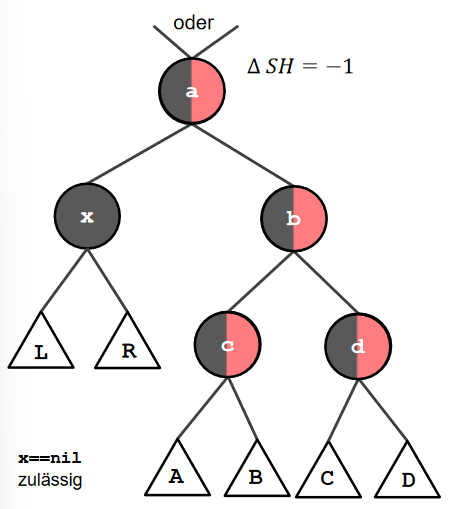
\includegraphics[width=0.5\textwidth]{Bilder/RSFixup.png}
                \caption{Zur Verdeutlichung}
                \label{fig:RSFixup}
            \end{figure}\\
            \newpage
            \begin{itemize}
                \item Fall I: a schwarz, b rot (wird zu Fall IIa, III oder IV, nie zu IIb)
                \item Fall IIa: a rot, b schwarz, c,d nicht rot (Wenn a rot, dann auf schwarz setzen und damit ursprüngliche SH erreicht)
                \item Fall IIb: a schwarz, b schwarz, c,d nicht rot (Wenn a schwarz, dann Vaterknoten $\triangle SH = \pm 1$; verfahre rekursiv mit a als neuem x)
                \item Fall III: a beliebig, b schwarz, c rot, d nicht rot (wird zu Fall IV)
                \item Fall IV: a beliebig, b schwarz, c beliebig, d rot (ursprüngliche SH wie zuvor)
            \end{itemize}
            \newpage
            \begin{figure}[ht]
                \centering
                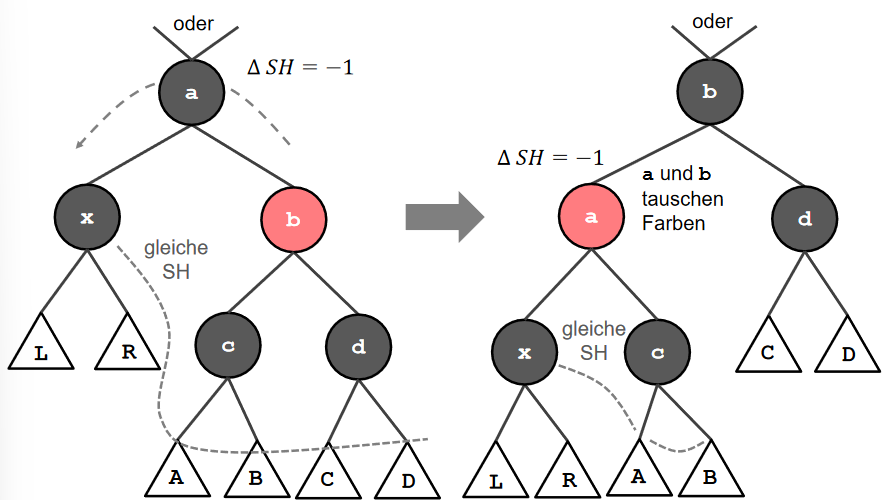
\includegraphics[width=0.5\textwidth]{Bilder/RSFixupI.png}
                \caption{FixUp Fall I}
                \label{fig:RSFixupI}
            \end{figure}
            \begin{figure}[ht]
                \centering
                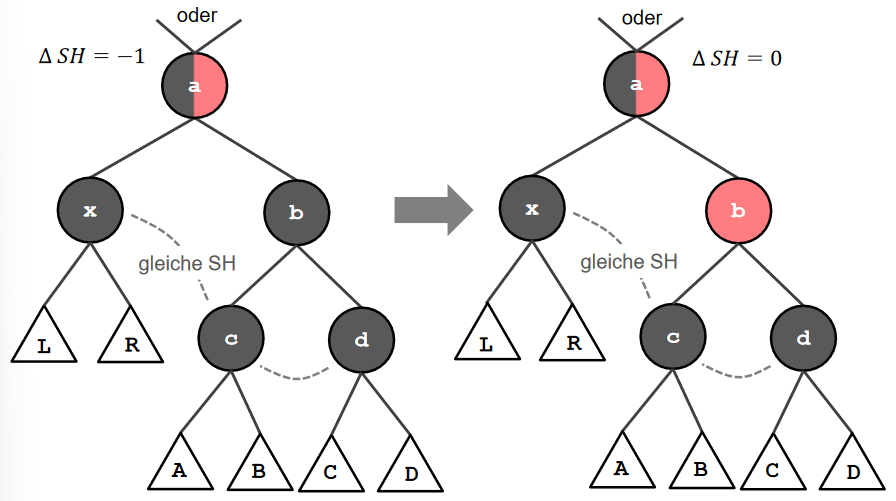
\includegraphics[width=0.5\textwidth]{Bilder/RSFixupIIa.png}
                \caption{FixUp Fall IIa}
                \label{fig:RSFixupIIa}
            \end{figure}
            \begin{figure}[ht]
                \centering
                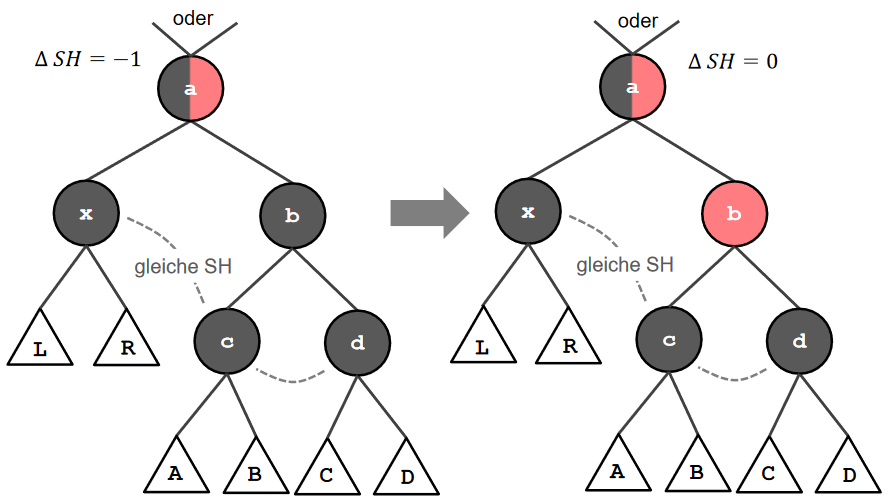
\includegraphics[width=0.5\textwidth]{Bilder/RSFixupIIb.png}
                \caption{Zur VerdeFixUp Fall IIb}
                \label{fig:RSFixupIIb}
            \end{figure}
            \begin{figure}[ht]
                \centering
                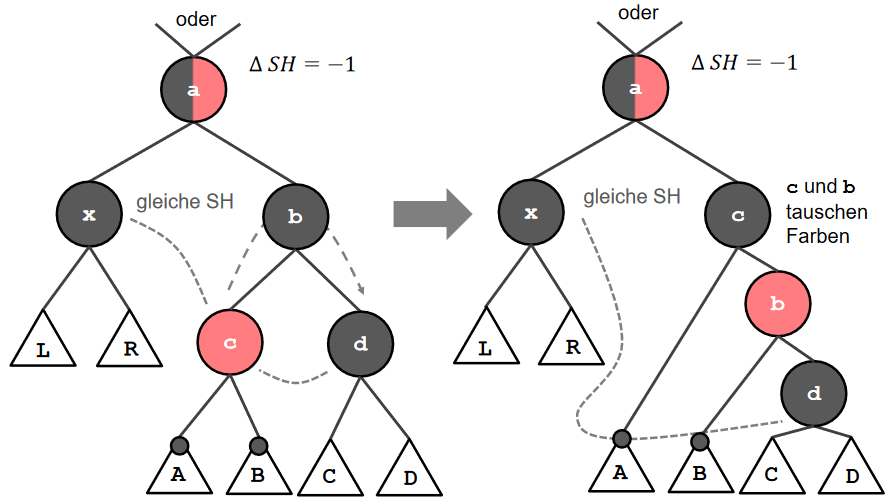
\includegraphics[width=0.5\textwidth]{Bilder/RSFixupIII.png}
                \caption{FixUp Fall III}
                \label{fig:RSFixupIII}
            \end{figure}
            \begin{figure}[ht]
                \centering
                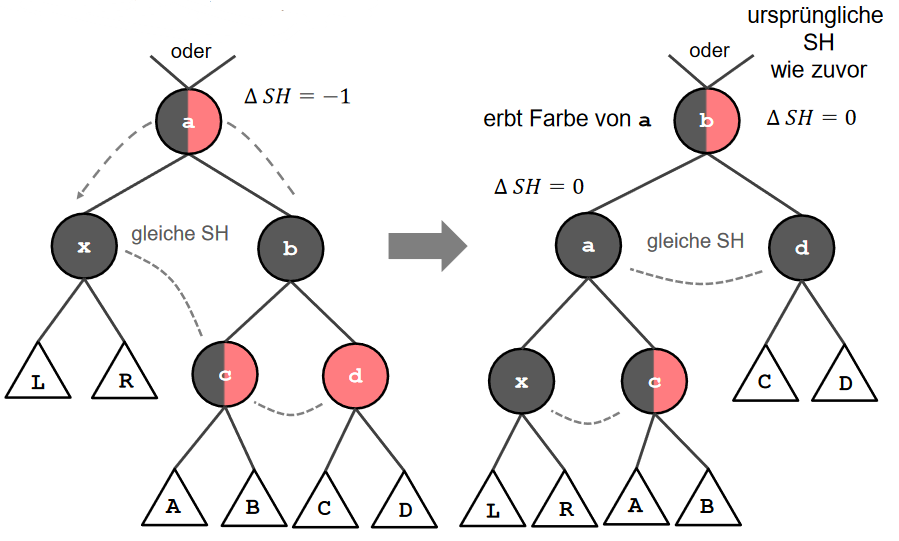
\includegraphics[width=0.5\textwidth]{Bilder/RSFixupIV.png}
                \caption{FixUp Fall IV}
                \label{fig:RSFixupIV}
            \end{figure}
            \newpage
            \textbf{Laufzeit:} $O(h) = O(log_n)$\\
            \textbf{Worst- Case- Laufzeiten:}\\
            \begin{itemize}
                \item Einfügen: $\Theta(log n)$
                \item Löschen: $\Theta(log n)$
                \item Suchen: $\Theta(log n)$
            \end{itemize}
        \subsection{AVL- Bäume}
            Benannt nach Georgi Maximowitsch Adelson-Velski und Jewgeni Michailowitsch Landis. \\
            Ein AVL-Baum ist ein binärer Suchbaum, so dass für die Balance $B(x)$ in jede Knoten x gilt: $B(x)\in{-1, 0, +1}$.\\
            Dabei ist $B(x)= \text{Höhe}(rechter Teilbaum)- \text{Höhe}(linker Teilbaum)$.\\
            Beispiel:
            \begin{figure}[ht]
                \centering
                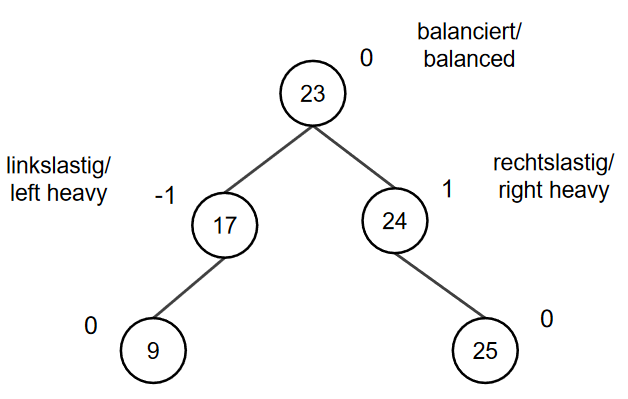
\includegraphics[width=0.5\textwidth]{Bilder/AVLEx.png}
                \caption{Beispiel}
                \label{fig:AVLEx}
            \end{figure}
            \newpage
            \textbf{Höhe AVL- Baum:} Sei $n_h$ minimale Anzahl von Knoten in einem AVL- Baum der Höhe h. Allgemein gilt für die Berechnung $n_h=1+n_{h-1}+n_{h-2}$.\\
            \begin{figure}[ht]
                \centering
                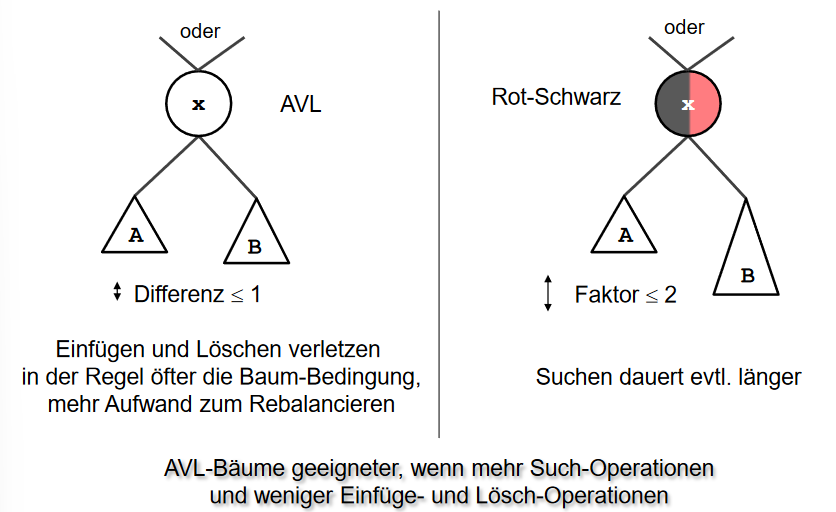
\includegraphics[width=1\textwidth]{Bilder/AVLvsRS.png}
                \caption{AVL vs. RS}
                \label{fig:AVLvsRS}
            \end{figure}\\
            Außerdem gilt: AVL $\subset$ Rot- Schwarz $\Rightarrow$ Jeder nicht-leere AVL-Baum der Höhe h lässt sich als Rot-Schwarz-Baum mit Schwarzhöhe $(h+1)/2$ darstellen.\\
            \begin{lstlisting}[style=pseudocode]
insert(T,z) //z.left==z.right==nil;
    x=T.root; px=T.sent;
    WHILE x != nil DO
        px=x;
        IF x.key > z.key THEN
            x=x.left
        ELSE
            x=x.right;
    z.parent=px;
    IF px==T.sent THEN
        T.root=z
    ELSE
        IF px.key > z.key THEN
            px.left=z
        ELSE
            px.right=z;
    fixBalanceAfterInsertion(T,z);
            \end{lstlisting}
            \textbf{Rebalancing:}
            \begin{figure}[ht]
                \centering
                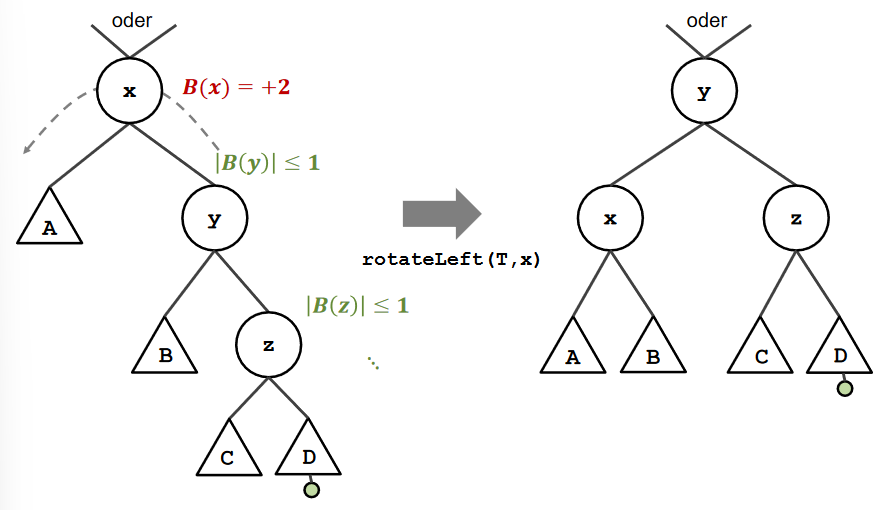
\includegraphics[width=0.75\textwidth]{Bilder/AVLRF1.png}
                \caption{Fall 1}
                \label{fig:AVLRF1}
            \end{figure}
            \begin{figure}[ht]
                \centering
                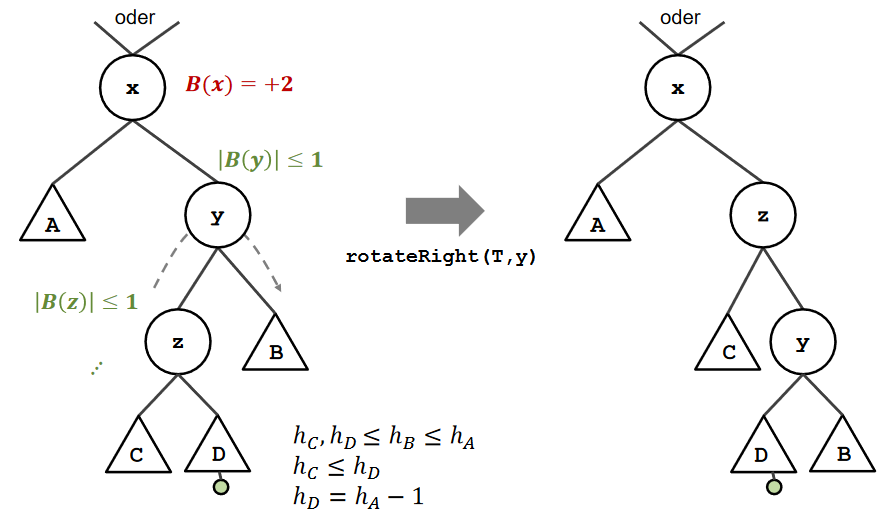
\includegraphics[width=0.75\textwidth]{Bilder/AVLRF2I.png}
                \caption{Fall 2, Teil 1}
                \label{fig:AVLRF2I}
            \end{figure}
            \begin{figure}[ht]
                \centering
                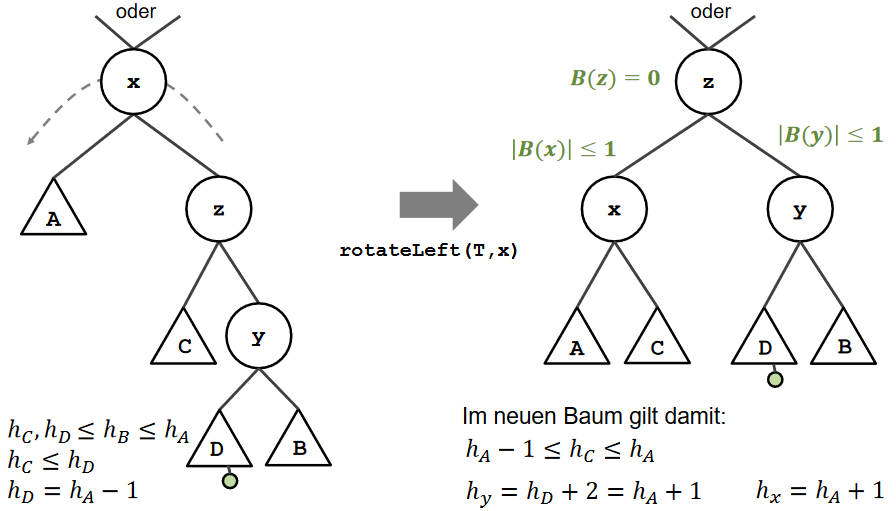
\includegraphics[width=0.75\textwidth]{Bilder/AVLRF2II.png}
                \caption{Fall 2, Teil 2}
                \label{fig:AVLRF2II}
            \end{figure}
            \begin{figure}[ht]
                \centering
                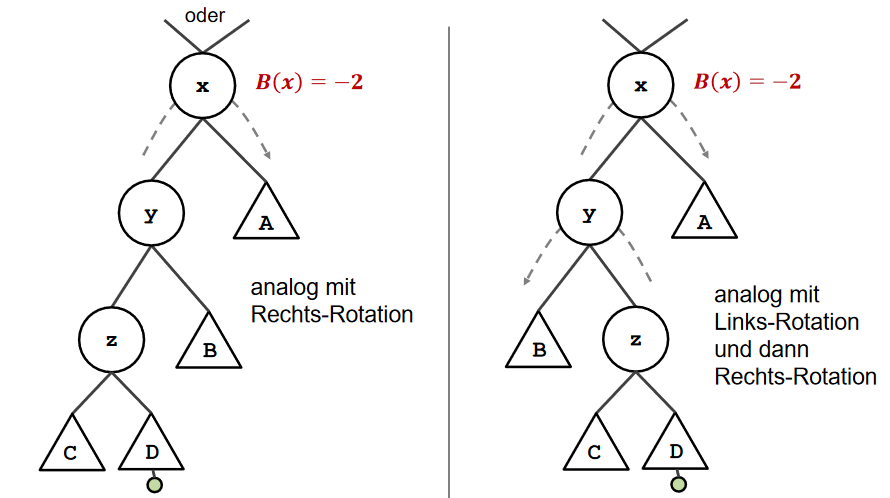
\includegraphics[width=0.75\textwidth]{Bilder/AVLRF3_4.png}
                \caption{Fall 3 und 4}
                \label{fig:AVLRF3_4}
            \end{figure}
            \newpage
            Löschen ist analog zu binären Suchbäumen, aber man muss das Rebalancing beachten.\\
            Allgemein haben wir hier auch selbe Laufzeit wie bei Rot- Schwarz- Bäumen.
        \subsection{Splay- Bäume}
            Splay Bäume sind selbst- organisierte Datenstrukturen, die den gesuchten Knoten an die Position der Wurzel schieben.\\
            Dabei gibt es die sogenannte Splay- Operation (\textbf{Laufzeit:} $O(h)$), die die Datenstruktur nach der oben genannten Regel verschiebt.
            \begin{lstlisting}[style=pseudocode]
splay(T,z)
    WHILE z != T.root DO
        IF z.parent.parent==nil THEN
            zig(T,z);
        ELSE
            IF z==z.parent.parent.left.left OR z==z.parent.parent.right.right THEN
                zigZig(T,z);
            ELSE
                zigZag(T,z);
            \end{lstlisting}
            \textbf{Laufzeit:} $O(h)$.\\
            Operationen:
            \begin{figure}[ht]
                \centering
                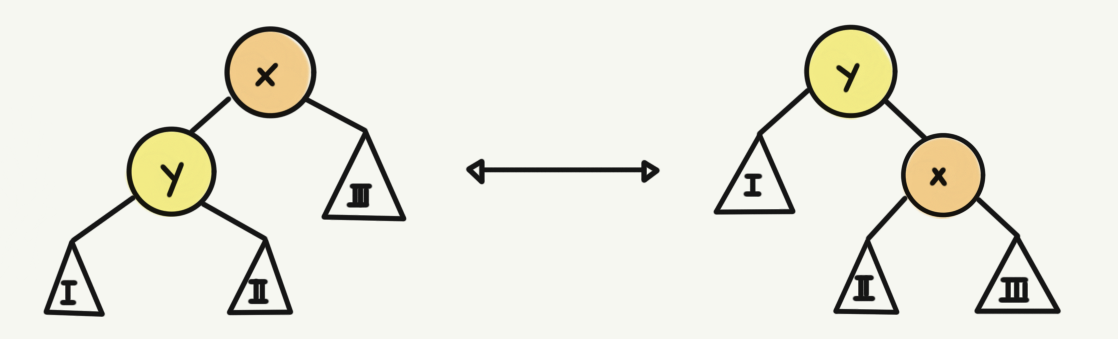
\includegraphics[width=0.75\textwidth]{Bilder/SplayZig.png}
                \caption{Zig- Operation}
                \label{fig:SplayBaeumeZig}
            \end{figure}
            \begin{figure}[ht]
                \centering
                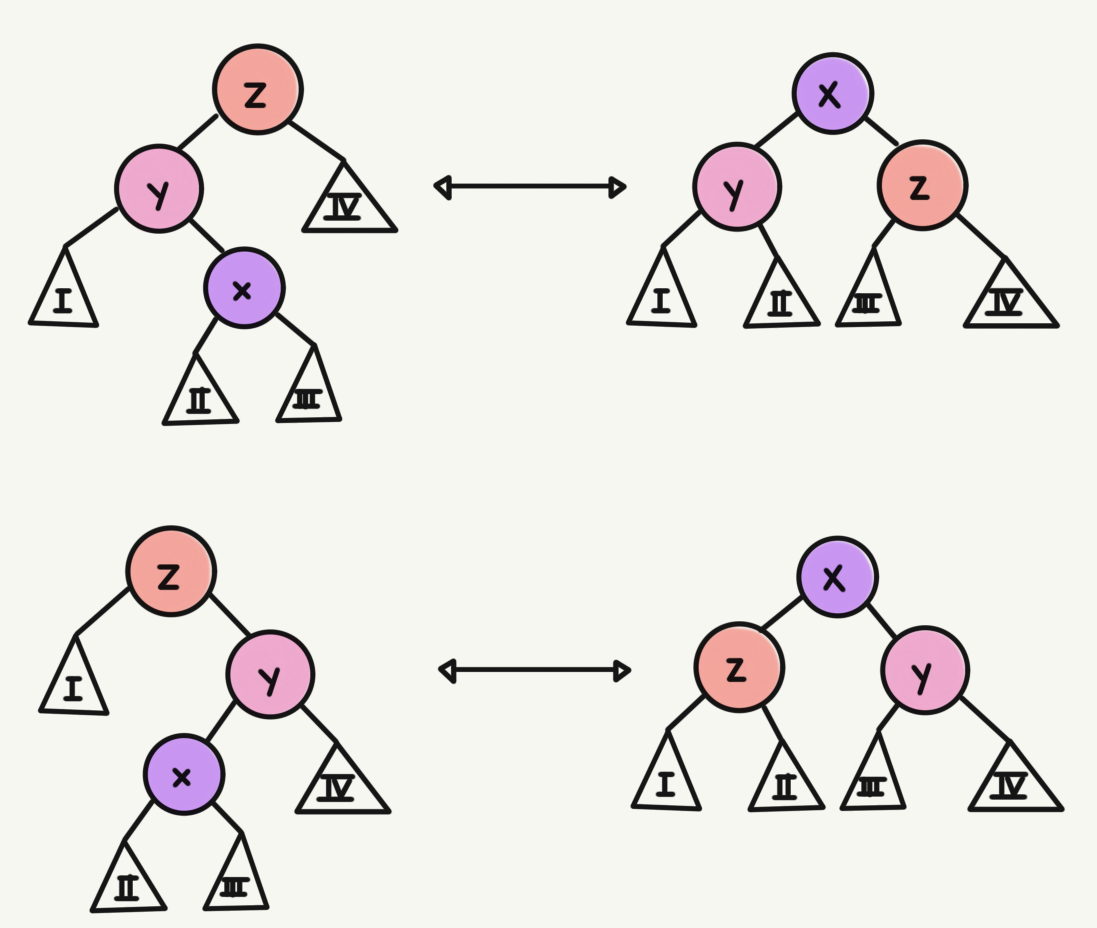
\includegraphics[width=0.75\textwidth]{Bilder/SplayZigZag.png}
                \caption{ZigZag- Operation}
                \label{fig:SplayBaeumeZigZag}
            \end{figure}
            \begin{figure}[ht]
                \centering
                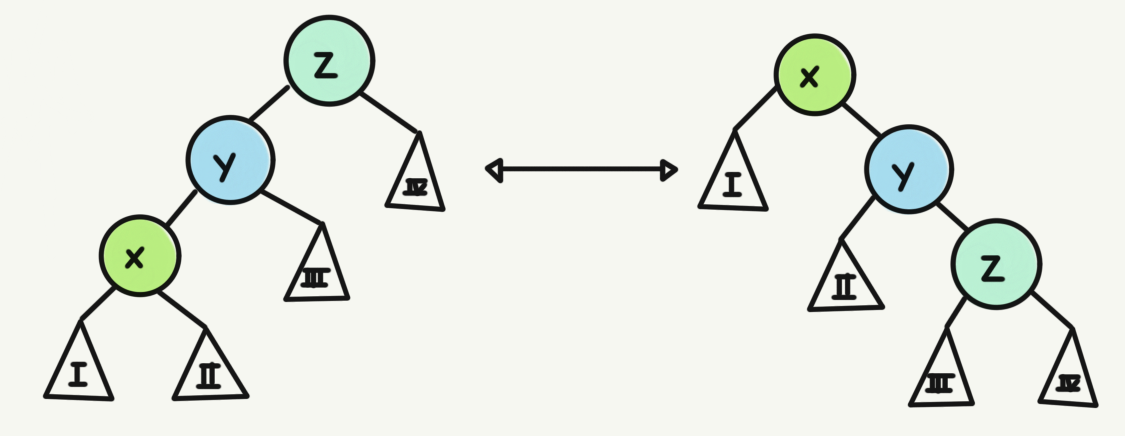
\includegraphics[width=0.75\textwidth]{Bilder/SplayZigZig.png}
                \caption{ZigZig- Operation}
                \label{fig:SplayBaeumeZigZig}
            \end{figure}
            \begin{lstlisting}[style=pseudocode]
zigZig(T,z)
    IF z==z.parent.left THEN
        rotateRight(T,z.parent.parent);
        rotateRight(T,z.parent);
    ELSE
        rotateLeft(T,z.parent.parent);
        rotateLeft(T,z.parent);
            \end{lstlisting}
            Zig und ZigZag Operationen werden analog implementiert. \\
            Suchen:
            \begin{lstlisting}[style=pseudocode]
search(T,k)
    x=T.root;
    WHILE x != nil AND x.key != k DO
        IF x.key < k THEN
            x=x.right
        ELSE
            x=x.left;
    IF x==nil THEN
        RETURN nil
    ELSE
        splay(T,x);
        RETURN T.root;
            \end{lstlisting}
            \textbf{Laufzeit:} $O(h)$.\\
            Einfügen: Analog zum BST wird der Knoten eingefügt und danach mithilfe der Splay Operation nach oben gespült.\\
            \textbf{Laufzeit:} $O(h)$.\\
            Löschen: Per Splay- Operation nach oben spülen. Dann löschen (Falls einer der beiden Kinderteilbäume leer, ist man fertig, sonst:)\\
            \begin{figure}[ht]
                \centering
                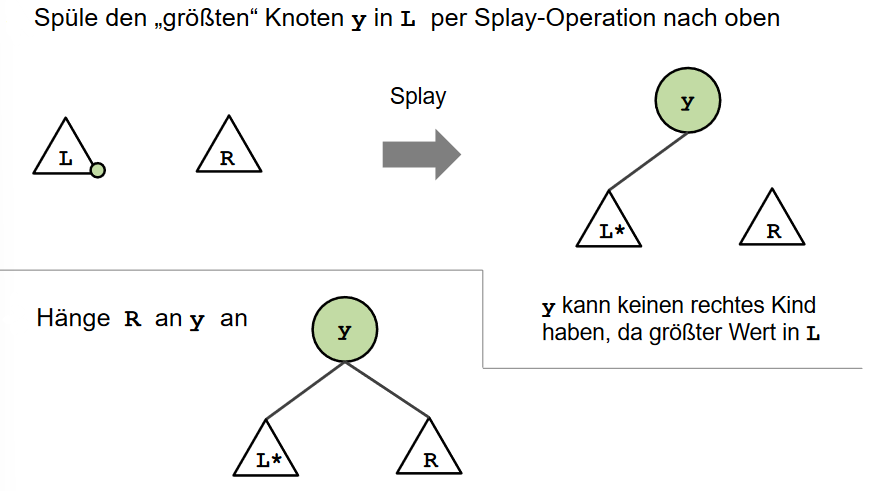
\includegraphics[width=0.75\textwidth]{Bilder/SplaynachL.png}
                \caption{Verschieben nach Löschen}
                \label{fig:SplaynachL}
            \end{figure}
            \newpage
        \subsection{(Binäre Max-) Heaps}
            Ein binärer Max-Heap ist ein binärer Baum, der
            \begin{itemize}
                \item 'Bis auf das unterste Level vollständig und im untersten Level von links gefüllt ist'
                \item Für alle Knoten x $\neq$ T.root gilt: x.parent.key $\geq$ x.key
            \end{itemize}
            \textbf{Achtung:} Heaps sind keine BSTs, linke Kinder können größere Werte als rechte Kinder haben!\\
            \begin{figure}[ht]
                \centering
                \includegraphics[width=0.75\textwidth]{Bilder/BspHeaps.png}
                \caption{Beispiel für einen Heap}
                \label{fig:BspHeaps}
            \end{figure}\\
            Ein Heap kann auch als Array dargestellt werden, in der von oben nach unten, von links nach rechhts in den Array eingefügt werden.\\
            Einfügen:\\
            Beim einfügen wird das Element an letzter Stelle eingfügt und so lange nach oben vertauscht, bis die Max- Eigenschaft wieder erfüllt ist.\\
            \begin{lstlisting}[style=pseudocode]
insert(H,k) //als (unbeschraenktes) Array
    H.length=H.length+1;
    H.A[H.length-1]=k;
    i=H.length-1;
    WHILE i>0 AND H.A[i] > H.A[i.parent]
        SWAP(H.A,i,i.parent);
        i=i.parent;
            \end{lstlisting}
            \textbf{Laufzeit:} $O(h) = O(log n)$. \\
            Löschen:\\
            1. Erste Maximum durch 'letztes' Blatt\\
            2.Stelle Max-Eigenschaften wieder her, indem Knoten nach unten gegen das Maximum der beiden Kinder getauscht wird (heapify)\\
            \begin{lstlisting}[style=pseudocode]
extract-max(H) //als (unbeschraenktes) Array
    IF isEmpty(H) THEN
        RETURN error 'underflow';
    ELSE
        max=H.A[0];
        H.A[0]=H.A[H.length-1];
        H.length=H.length-1;
        heapify(H,0);
        RETURN max;
            \end{lstlisting}
            \textbf{Laufzeit:} $O(h) = O(log n)$.
            \begin{lstlisting}[style=pseudocode]
heapify(H,i) //als (unbeschraenktes) Array
    maxind=i;
    IF i.left<H.length AND H.A[i]<H.A[i.left] THEN
        maxind=i.left;
    IF i.right<H.length AND H.A[maxind]<H.A[i.right] THEN
        maxind=i.right;
    IF maxind != i THEN
        SWAP(H.A,i,maxind);
        heapify(H,maxind);
            \end{lstlisting}
            \textbf{Laufzeit:} $O(h) = O(log n)$. \\
            Heap- Konstruktion: \\
            \begin{lstlisting}[style=pseudocode]
buildHeap(H) //Array A schon nach H.A kopiert
    H.length=A.length;
    FOR i = ceil((H.length-1)/2)-1 DOWNTO 0 DO
        heapify(H,i);
            \end{lstlisting}
            \textbf{Laufzeit:} $O(n\cdot h) = O(n\cdot log n)$.\\
            Heap- Sort:\\
            \begin{lstlisting}[style=pseudocode]
heapSort(H) //Array A schon nach H.A kopiert
    buildHeap(H);
    WHILE !isEmpty(H) DO PRINT extract-max(H) //Gibt Eintraege in Array A in absteigender Groesse aus
            \end{lstlisting}
            \textbf{Laufzeit:} $O(n\cdot h) = O(n\cdot log n)$.\\
            In Java können diese mit Priority Queues dargestellt werden.
        \subsection{B- Bäume}
            Ein B-Baum (vom Grad t) ist ein Baum, bei dem
            \begin{itemize}
                \item Jeder Knoten (außer der Wurzel) zwischen t - 1 und 2t - 1 Werte key[0],key[1],… hat und die Wurzel zwischen 1 und 2t - 1
                \item Die Werte innerhalb eines Knoten aufsteigend geordnet sind
                \item Die Blätter alle die gleiche Höhe haben
                \item jeder innerer Knoten mit n Werten n + 1 Kinder hat, so dass für alle Werte $k_j$ aus dem j-ten Kind gilt: \\$k_o \leq key[0] \leq k_1 \leq key[1] \leq ... \leq k_{n-1} \leq key[n-1] \leq k_n$.
            \end{itemize}
            Beispiel:
            \begin{figure}[ht]
                \centering
                \includegraphics[width=0.75\textwidth]{Bilder/BB.png}
                \caption{Beispiel B- Baum}
                \label{fig:BB}
            \end{figure}\\
            Für die Höhe gilt:
            \begin{itemize}
                \item mindestens 1 Wert in Wurzel
                \item mindestens 2 Knoten in Tiefe 1 mit jeweils mindestens t Kindern
                \item mindestens 2t Knoten in nächster Tiefe mit jeweils mindestens t Kindern
                \item mindestens $2t^2$ Knoten in nächster Tiefe mit jeweils mindestens t Kindern, usw.
            \end{itemize}
            Anzahl Werte n im B-Baum im Vergleich zu Höhe : $n \geq 1+(t-1)\cdot \sum_{i=1}^{h}2t^{i-1}=1+2(t-1)\cdot \frac{t^h-1}{t-1}=2t^h-1 \Rightarrow log_t \frac{n+1}{2} \geq h$.\\
            Ein B-Baum vom Grad t mit n Werten hat maximale Höhe $h \leq log_t \frac{n+1}{2}$.\\
            Suchen:
            \begin{lstlisting}[style=pseudocode]
search(x,k)
    WHILE x != nil DO
        i=0;
        WHILE i < x.n AND x.key[i] < k DO i=i+1;
        IF i < x.n AND x.key[i]==k THEN
            RETURN (x,i);
        ELSE
            x=x.child[i];
    RETURN nil; 
            \end{lstlisting}
            \textbf{Laufzeit:} $O(t\cdot h) = O(log_t n)$.\\
            Einfügen: Immer in einem Blatt. Wenn das Blatt dabei weniger als $2t-1$ Werte hat, sind wir fertig, sonst müssen wir splitten:\\
            \begin{figure}[ht]
                \centering
                \includegraphics[width=0.75\textwidth]{Bilder/SplittenBB.png}
                \caption{Splitten B- Baum}
                \label{fig:SplittenBB}
            \end{figure}
            Sollte die Wurzel voll sein, wird diese gesplittet.\\
            \begin{lstlisting}[style=pseudocode]
insert(T,z)
    Wenn Wurzel schon 2t-1 Werte, dann splitte Wurzel
    Suche rekursiv Einfuegeposition:
        Wenn zu besuchendes Kind 2t-1 Werte, splitte es erst
    Fuege z in Blatt ein
            \end{lstlisting}
            Löschen:\\
            Löschen funktioniert intuitiv.\\
            \begin{figure}[ht]
                \centering
                \includegraphics[width=0.75\textwidth]{Bilder/BBdel1.png}
                \caption{Löschen im 'zu leeren' Blatt: Rotieren}
                \label{fig:BBdel1}
            \end{figure}\\
            \begin{figure}[ht]
                \centering
                \includegraphics[width=0.75\textwidth]{Bilder/BBdel2.png}
                \caption{Löschen im 'zu leeren' Blatt: Verschmelzen}
                \label{fig:BBdel2}
            \end{figure}\\
            \begin{figure}[ht]
                \centering
                \includegraphics[width=0.725\textwidth]{Bilder/BBdel3.png}
                \caption{Löschen im inneren Knoten: Verschieben}
                \label{fig:BBdel3}
            \end{figure}
            \begin{figure}[ht]
                \centering
                \includegraphics[width=0.725\textwidth]{Bilder/BBdel4.png}
                \caption{Löschen im inneren Knoten: Verschmelzen}
                \label{fig:BBdel4}
            \end{figure}
            \newpage
            \begin{lstlisting}[style=pseudocode]
delete(T,k)
    Wenn Wurzel nur 1 Wert und beide Kinder t-1 Werte, verschmelze Wurzel und Kinder (reduziert Hoehe um 1)
    Suche rekursiv Loeschposition:
        Wenn zu besuchendes Kind nur t-1 Werte, verschmelze es oder rotiere/verschiebe
    Entferne Wert k in inneren Knoten/Blatt
            \end{lstlisting}
            \textbf{Laufzeit:} $O(t\cdot h) = O(log_t n)$.\\
            Worst- Case- Laufzeiten: 
            \begin{itemize}
                \item Einfügen/ Löschen/ Suchen: $\Theta(log_t n)$.
            \end{itemize}

    \newpage
    \section{Randomized Data Structures}
        \subsection{Skip- Lists}
            Eine Skip Liste ist eine Liste, in der eine 'Express- Liste' mit einigen Elementen ist.\\
            \begin{figure}[ht]
                \centering
                \includegraphics[width=0.75\textwidth]{Bilder/Skip.png}
                \caption{Beispiel einer Skip- Liste}
                \label{fig:Skip}
            \end{figure}\\
            Mann kann auch mehrere immer kleinere Express- Listen über der Express- Liste einbauen.\\
            Suchen funktioniert hierbei nach dem folgenden Muster:
            \begin{itemize}
                \item Element gefunden? → Element ausgeben
                \item Nächstes Element in Express-Liste kleiner-gleich gesuchtes Element? → Weiter nach rechts
                \item Nächstes Element in Express-Liste größer als gesuchtes Element? → Nach unten in ursprüngliche Liste und dort weitersuchen
            \end{itemize}
            Dabei werden die Elemente auf jeder Express- Ebene zufällig mit einer Wahrscheinlichkeit von $p$ gewählt.
            Implementierung:
            \begin{itemize}
                \item L.head - erstes/oberstes Element der Liste
                \item L.height - Höhe der Skiplist
                \item x.key - Wert
                \item x.next - Nachfolger
                \item x.prev - Vorgänger
                \item x.down - Nachfolger Liste unten
                \item x.up - Nachfolger Liste oben
                \item nil - kein Nachfolger / leeres Element
            \end{itemize}
            \begin{lstlisting}[style=pseudocode]
search(L,k)
    current=L.head;
    WHILE current != nil DO
        IF current.key == k THEN RETURN current;
        IF current.next != nil AND current.next.key <= k
        THEN current=current.next
        ELSE current=current.down;
    RETURN nil;
            \end{lstlisting}
            Durchschnittliche \textbf{Laufzeit:} $O(h)$, jedoch abhängig von der größe der Expresslisten.\\
            \textbf{Einfügen:} In der untersten Ebene einfügen und dann per Wahrscheinlichkeit $p$ in die darüber einfügen. (Durchschnittliche \textbf{Laufzeit:} $O(h)$)\\ 
            \textbf{Löschen:} Entferne Vorkommen des Elements auf allen Ebenen (\textbf{Laufzeit:} $O(h)$)\\
            Worst- Case- Laufzeiten (in Durchschnitt): $\Theta(log_{1/p}n)$.
        \subsection{Hash- Tables}
            Idee:\\
            \begin{figure}[ht]
                \centering
                \includegraphics[width=0.75\textwidth]{Bilder/HashTIdee.png}
                \caption{Grundkonzept eines Hash- Tables}
                \label{fig:HashTIdee}
            \end{figure}\\
            \textbf{Einfügen:} Wir schauen, ob $w$ in $T[h(w)]$ vorhanden ist (search(H,w))\\
            \textbf{Löschen:} Intuitiv (delete(H,z))\\
            Dabei erfolgt suchen/ löschen mit konstant vielen Array- Operation\\
            \textbf{Kolisionsauflösung:} Falls ein Eintrag im Array schon belegt ist, bildet man eine verkettete Liste und fügt neues Element vorne ein.\\
            Daraus folgt dann:
            \begin{figure}[ht]
                \centering
                \includegraphics[width=0.5\textwidth]{Bilder/HashTVL.png}
                \caption{Hash- Tabelle als verkettete Liste}
                \label{fig:HashTVL}
            \end{figure}
            \newpage
            Einfügen immer noch konstante Anzahl Array-/Listen-Operationen.\\
            Wenn Hashfunktion uniform verteilt, dann hat jede Liste im Erwartungswert $frac{n}{T.length}$ viele Einträge.\\
            Worst- Case- \textbf{Laufzeiten:} (Im Durchschnitt)
            \begin{itemize}
                \item Einfügen: $\Theta(1)$
                \item Löschen: $\Theta(1)$
                \item Suchen: $\Theta(1)$
            \end{itemize}
        \subsection{Bloom- Filter}
            Beispiel: Speichere ('offline') alle schlechten Passwörter im Bloom-Filter. Prüfe ('online'), ob eingegebenes Passwort im Bloom-Filter.\\
            Anwendungsbeispiel: Bitcoin (Prüfen von Transaktionen); NoSQL- DB (Abfragen für nicht vorhandene ELemente verhindern).\\
            
            \textbf{Filter erstellen:}\\
            Gegeben: 
            \begin{itemize}
                \item $n$ Elemente $x_0...,x_{n-1} $beliebiger Komplexität
                \item $m$ Bits Speicher, üblicherweise in einem Bit-Array
                \item $k$ 'gute' Hash-Funktionen $H_0,...,H_{k-1}$ mit Bildbereich $0,1,...,m-1$
            \end{itemize}
            Empfohlen wird jedoch: $k=\frac{m}{n}\cdot ln2$.\\
            \begin{lstlisting}[style=pseudocode]
initBloom(X,BF,H) //H array of functions H[j]
FOR i=0 TO BF.length-1 DO BF[i]=0;
FOR i=0 TO X.length-1 DO
    FOR j=0 TO H.length-1 DO
        BF[H[j](X[i])]=1;
            \end{lstlisting}
            1. Inititalisierte Array mit 0 Einträgen.\\
            2. Schreibe für jedes Element in jede Bit-Position $H_0(x_i),...,H_{k-1}(x_i)$ eine 1. \\
            \begin{figure}[ht]
                \centering
                \includegraphics[width=1\textwidth]{Bilder/Bloom.png}
                \caption{Visualisierung}
                \label{fig:Bloom}
            \end{figure}\\
            \textbf{Suchen:}
            \begin{lstlisting}[style=pseudocode]
searchBloom(BF,H,y) //H array of functions H[j]
    result=1;
    FOR j=0 TO H.length-1 DO
        result=result AND BF[H[j](y)];
    RETURN result;
            \end{lstlisting}
            Gibt an, dass y im Wörterbuch, wenn genau alle k Einträge für y in BF=1 sind.

    \newpage
    \section{Graph Algorithms}
        \subsection{Graphen}
            \textbf{(Endliche) Gerichtete Graphen:}\\
            Ein (endlicher) gerichteter Graph G = (V, E) besteht aus:
            \begin{itemize}
                \item einer (endlichen) Knotenmenge V ('vertices')
                \item einer (endlichen) Kantenmenge E $\subseteq$ V x V ('edges')
            \end{itemize}
            Dabei ist $(u,v)\in E$ Kante von Knoten u zu v.\\
            Außerdem können keine Mehrfachkanten zwischen Knoten existieren. \\
            Beispiel:
            \begin{figure}[ht]
                \centering
                \includegraphics[width=0.75\textwidth]{Bilder/GeGraphBSP.png}
                \caption{Beispiel}
                \label{fig:GeGraphBSP}
            \end{figure}\\
            \textbf{Ungerichtete Graphen:}\\
            Ein ungerichteter Graph G = (V, E) besteht aus:
            \begin{itemize}
                \item einer (endlichen) Knotenmenge V ('vertices')
                \item einer (endlichen) Kantenmenge E $\subseteq$ V x V ('edges'), so dass $(u,v)\in E \Leftrightarrow (v,u)\in E$
            \end{itemize}
            Man kann Graphen auch as ${u,v} statt (u,v),(v,u)$ darstellen.\\
            \begin{figure}[ht]
                \centering
                \includegraphics[width=0.75\textwidth]{Bilder/UgGraphBSP.png}
                \caption{Beispiel}
                \label{fig:UgGraphBSP}
            \end{figure}\\
            Dabei gilt: $shortest(u,v)$= Länge eines kürzestens Pfades von u nach v,\\
            \textbf{Zusammenhänge:}
            \begin{itemize}
                \item Ungerichteter Graph ist \textbf{zusammenhängend}, wenn jeder Knoten von jedem anderen Knoten aus erreichbar ist
                \item Gerichteter Graph ist \textbf{stark zusammenhängend}, wenn jeder Knoten von jedem anderen Knoten aus (gemäß Kantenrichtung) erreichbar ist
            \end{itemize}
            Graph G = (V, E) ist ein Baum, wenn V leer ist oder es einen Knoten $r\in V$ ('Wurzel') gibt, so dass jeder Knoten v von der Wurzel aus per eindeutigem Pfad erreichbar ist.\\
            (Gerichteter oder ungerichteter) Graph G' = (V', E') ist Subgraph (oder Untergraph oder Teilgraph) des (gerichteten oder ungerichteten) Graphen G = (V, E), wenn V' $\subseteq$ V und E' $\subseteq$ E.\\
            Man kann diese auch als Graphen darstelle (Speicherbedarf $\Theta(|V|^2)$). 
            \begin{figure}[ht]
                \centering
                \includegraphics[width=0.5\textwidth]{Bilder/Matrix.png}
                \caption{Matrix und Regeln}
                \label{fig:Matrix}
            \end{figure}\\
            \newpage
            \textbf{Matrixeigenschaften:} Der Eintrag $a_{i,j}^{(m)}$ in der i-ten Zeile und j-ten Spalte der m-ten Potenz $A^m$ der Adjazenzmatrix A eines Graphen gibt die Anzahl der Wege an, die von Knoten i zu Knoten j entlang von genau m Kanten führen (m $\geq$ 0).\\
            \textbf{Gewichteter Graph:} Ein gewichteter gerichteter Graph G = (V, E) besitzt zusätzlich Funktion $w: E \rightarrow R$ Bei gewichteten ungerichteten Graphen gilt zusätzlich $w=((u,v)) = w((v,u))$ für alle $(u,v)\in E$.
        \subsection{BFS (Breadth- First- Search)}
            Idee: Besuche zuerst alle unmittelbaren Nachbarn, dann deren Nachbarn usw...\\
            Dabei bekommt jeder Knoten eine Farbe zugeordnet.
            \begin{itemize}
                \item WHITE = Knoten noch nicht besucht
                \item GRAY = in Queue für nächsten Schritt
                \item BLACK = fertig
            \end{itemize}
            \begin{lstlisting}[style=pseudocode]
BFS(G,s) //G=(V,E), s=source node in V
    FOREACH u in V-{s} DO
        u.color=WHITE; u.dist=+infinit; u.pred=NIL;
    s.color=GRAY; s.dist=0; s.pred=NIL;
    newQueue(Q);
    enqueue(Q,s);
    WHILE !isEmpty(Q) DO
        u=dequeue(Q);
        FOREACH v in adj(G,u) DO
            IF v.color==WHITE THEN
                v.color=GRAY; v.dist=u.dist+1; v.pred=u;
                enqueue(Q,v);
        u.color=BLACK;
            \end{lstlisting}
            Dabei ist \textit{dist} = Distanz von s \& \textit{pred} = Vorgängerknoten \& \textit{adj(G,u)} = Liste aller Knoten $v \in V$ mit $(u,v) \in E$ (Rheinenfolge irrelevant).\\
            \textbf{Erklärung:} Jeder Knoten hat zu Beginn keinen Vorgänger und Entfernung unendlich. Begonnen wird mit dem Starkknoten, der alle Knoten abläuft und sich selber als Vorgänger (mit der Entfernung) einträgt und diese zum Ablaufen einfärbt.
            Danach wird mit diesen Knoten weiter verfahren, bis die Queue Q leer ist.\\
            \begin{figure}[ht]
                \centering
                \includegraphics[width=0.75\textwidth]{Bilder/BFSAlg.png}
                \caption{Besipiel für den Beginn des Algorithmus}
                \label{fig:BFSAlg}
            \end{figure}\\
            Hierbei werden immer die abgearbeitet, die zuerst in der Queue waren. Bei Adding in der gleichen Iteration, wird zuerst das mit dem kleineren Index abgelaufen.\\
            \textbf{Laufzeit:} $O(|V|+|E|)$, insgesamt werden maximal $\sum_{u\in V}|adj(G,u)| = O(|E|)$ Kanten betrachtet.\\
            Algorithmus, um den kürzesten Pfad auszugeben:\\
            \begin{lstlisting}[style=pseudocode]
PRINT-PATH(G,s,v) //assumes that BFS(G,s) has already been executed
    IF v==s THEN
        PRINT s;
    ELSE
        IF v.pred==NIL THEN
            PRINT 'no path from s -> v';
        ELSE
            PRINT-PATH(G,s,v.pred);
            PRINT v;
            \end{lstlisting}
            \textbf{Laufzeit:} $O(|V|)$ (ohne BFS).\\
            \textbf{Abgeleiteter BFS- Baum:}\\
            $G^s_{pred}$ ist BFS- Baum zu G, d.h.enthält alle von s aus erreichbaren Knoten in G und für jeden Knoten v$\in V^s_{pred}$ existiert genau ein Pfad von s in $G^s_{pred}$, der auch ein kürzester Pfad von s zu v in G ist.
            Definition: 
            \begin{itemize}
                \item $G^s_{pred} = (V^s_{pred}, E^s_{pred})$
                \item $V^s_{pred} = \{v\in V|v.pred\neq NIL\} \cup {s}$
                \item $E^s_{pred} = \{ (v.pred,v) | v \in V^s_{pred} -\{s\}$
            \end{itemize}
            (Für ungerichtete Graphen: $(v,v.pred)$)
            \begin{figure}[ht]
                \centering
                \includegraphics[width=0.75\textwidth]{Bilder/BFSAbg.png}
                \caption{Beispiel für den Beginn des Algorithmus}
                \label{fig:BFSAbg}
            \end{figure}
        \subsection{DFS (Depth- First- Search)}
            Idee: Besuche zuerst alle noch nicht besuchten Nachfolgeknoten ('Laufe so weit wie möglich weg von aktuellem Knoten')\\
            \begin{lstlisting}[style=pseudocode]
DFS(G) //G=(V,E)
    FOREACH u in V DO
        u.color=WHITE;
        u.pred=NIL;
    time=0;
    FOREACH u in V DO
        IF u.color==WHITE THEN
            DFS-VISIT(G,u);
            \end{lstlisting}
            Dabei ist $time$ eine globale Variable.
            \begin{lstlisting}[style=pseudocode]
DFS-VISIT(G,u)
    time=time+1;
    u.disc=time;
    u.color=GRAY;
    FOREACH v in adj(G,u) DO
        IF v.color==WHITE THEN
            v.pred=u;
            DFS-VISIT(G,v);
    u.color=BLACK;
    time=time+1;
    u.finish=time;
            \end{lstlisting}
            Dabei ist $disc$ die discovery time und $finish$ die finish time. \\
            Beispiel:\\
            \begin{figure}[ht]
                \centering
                \includegraphics[width=0.5\textwidth]{Bilder/DFSBsp.png}
                \caption{Der Baum für das Beispiel}
                \label{fig:DFSBsp}
            \end{figure}
            \begin{figure}[ht]
                \centering
                \includegraphics[width=0.75\textwidth]{Bilder/DFSTab.png}
                \caption{Die daraus resultierende Tabelle}
                \label{fig:DFSTab}
            \end{figure}\\
            \textbf{Abgeleiteter DFS- Baum:}\\
            Subgraph $G_{pred} (V, E_{pred})$ von G mit $E_{pred}=\{(v.pred, v)| v \in V, v.pred \neq NIL \}$ ((v,v.pred) für ungerichtete Graphen). (DFS Baum gibt dabei nicht unbegint den kürzesten Pfad wieder)\\
            \textbf{Kanten zeigen} (Zeichne restlichen Kanten aus G auch in $G_{pred}$ ein).
            \begin{figure}[ht]
                \centering
                \includegraphics[width=1\textwidth]{Bilder/DFSAbg.png}
                \caption{Kanten zeigen}
                \label{fig:DFSAbg}
            \end{figure}
            \newpage
            \textbf{Kantenart erkennen:} Es gibt hierbei für gerichtete Graphen 4 verschiedene Fälle:\\
            Sei $(u,v)$ die gerade betrachtete Kante im DFS- Algorithmus. Dann ist $(u,v)$...
            \begin{itemize}
                \item \dots\textbf{eine Baumkante, wenn v.color==WHITE} \textit{(v noch nicht besucht, v.pred=u $\Rightarrow$ (v.pred,v)=(u,v) als Kante in $G_{pred}$)}
                \item \dots\textbf{eine Rückwärtskante, wenn v.color==GRAY} \textit{(die Kette von grauen Knoten, die auch im DFS-Baum eine Kette bilden)}
                \item \dots\textbf{eine Vorwärtskante, wenn v.color==BLACK und u.disc$<$v.disc} \textit{(da u.disc$<$v.disc wurde v schwarz, als u schon grau war; aber u ist noch nicht abgeschlossen, also wurde v von einem echten Nachkomme von u besucht, da u vorher zu einem weißen Knoten überging)}
                \item \dots\textbf{eine Kreuzkante, wenn v.color==BLACK und v.disc$<$u.disc} \textit{(alle anderen)}
            \end{itemize}
            \subsubsection{Anwendung}
                BFS: Web Crawling, Kontakte in OSN, Broadcasting, Garbage Collection\\
                DFS: Job Scheudling (In welcher Rheinenfolge sollen Jobs bearbeitet werden)\\
                Topologische Sortierung eines dag $G=(V,E)$: Knoten in linearer Ordnung, so dass für alle Knoten $u,v\in V$ gilt, dass $u$ vor $v$ in der Ordnung kommt, wenn $(u,v)\in E$.
                \begin{lstlisting}[style=pseudocode]
TOPOLOGICAL-SORT(G) // G=(V,E) dag
    newLinkedList(L);
    run DFS(G) but, each time a node is finished, insert in front of L;
    RETURN L.head;
                \end{lstlisting}
                \textbf{Laufzeit:} $O(|V|+|E|)$.\\
                \textbf{Starke Zusammenhangskomponente:}Eine starke Zusammenhangskomponente eines gerichteten Graphen $G=(V,E)$ ist eine Knotenmenge $C\subseteq V$, so dass\\
                (a) es zwischen je zwei Knoten $u,v\in C$ einen Pfad von $u$ nach $v$ gibt, und\\
                (b) es keine Menge $D\subseteq V$ mit $C !\subseteq D$ gibt, für die (a) auch gilt\\
                (C ist maximal).\\
                \begin{figure}[ht]
                    \centering
                    \includegraphics[width=0.75\textwidth]{Bilder/SZK.png}
                    \caption{Starke Zusammenhangskomponente Visualisierung}
                    \label{fig:SZK}
                \end{figure}\\
                \begin{figure}[ht]
                    \centering
                    \includegraphics[width=0.8\textwidth]{Bilder/SZKEig.png}
                    \caption{Eigenschaften}
                    \label{fig:SZKEig}
                \end{figure}\\
                Lasse zweimal DFS laufen:
                \begin{itemize}
                    \item einmal auf Graph G
                    \item einmal auf transponiertem Graphen $G^T = (V,E^T)$ ($E^T=\{(v,u)|(u,v)\in E\}$)
                \end{itemize}
                SCCs in $G$ und $G^T$ bleiben identisch (in beiden Fällen gibt es in jeder SCC einen Weg von jedem Knoten zum anderen Knoten), nur Übergänge zwischen SCCs drehen sich um.
                \begin{lstlisting}[style=pseudocode]
SCC(G) // G=(V,E) directed graph
    run DFS(G)
    compute G^T
    run DFS(G^T) but visit vertices in main loop in descending finish time from 1
    output each DFS tree in 3 as one SCC
                \end{lstlisting}
                \begin{figure}[ht]
                    \centering
                    \includegraphics[width=1\textwidth]{Bilder/Algorithmendesign.png}
                    \caption{Eigenschaften}
                    \label{fig:Algorithmendesign}
                \end{figure}
        \subsection{Minimale Spannbäume (MST)}
            Für einen zusammenhängenden, ungerichteten, gewichteten Graphen $G=(V,E)$ mit Gewichten $w$ ist der Subgraph $T=(V,E_T)$ von $G$ ein Spannbaum ('spanning tree'), wenn $T$ azyklisch ist und alle Knoten verbindet. \\
            Der Spannbaum ist minimal, wenn $w(T)=\sum_{\{u,v\}\in E_T}w(\{u,v\})$ minimal für alle Spannbäume von $G$ ist.\\
            \begin{figure}[ht]
                \centering
                \includegraphics[width=0.5\textwidth]{Bilder/MSTBsp.png}
                \caption{Beispiel}
                \label{fig:MSTBsp}
            \end{figure}
            Idee:\\
            \begin{lstlisting}[style=pseudocode]
genericMST(G,w) // G=(V,E) undirected, connected graph w weight function
    A={};
    WHILE A does not form a spanning tree for G DO
        find safe edge {u,v} for A;
        A = A vereinigt {{u,v}};
    RETURN A;
            \end{lstlisting}
            A: Teilmenge der Kanten eines MST; Kante $\{u,v\}$ ist sicher ('safe') für $A$, wenn $A \cup \{\{u,v\}\}$ noch eine Teilmenge eines MST ist.\\
            \textbf{Terminierung:} Da wir zeigen werden, dass es in jeder Iteration eine sichere Kante für $A$ gibt (sofern $A$ noch kein Spannbaum), terminiert die Schleife nach maximal $|E|$ Iterationen.\\
            \textbf{Korrektheit:} Da in jeder Iteration nur sichere Kanten hinzugefügt werden (für die $A \cup \{\{u,v\}\}$ noch Teilmenge eines MST ist), ist am Ende der WHILE-Schleife $A$ ein MST.\\
            \begin{figure}[ht]
                \centering
                \includegraphics[width=0.75\textwidth]{Bilder/MSTTerminologie.png}
                \caption{Terminologie udn Leicht=Sicher?}
                \label{fig:MSTTerminologie}
            \end{figure}
            'Leicht=sicher' legt Greedy- Strategie für konkrete Implementierung nahe. Daraus folgen zwei Ansätze:
            \begin{itemize}
                \item Algorithmus von Kruskal (lässt parallel mehrere Unterbäume eines MST wachsen)
                \item Algorithmus von Prim (konstruiert einen MST Knoten für Knoten)
            \end{itemize}
            \subsubsection{Kruskal}
                \begin{lstlisting}[style=pseudocode]
MST-Kruskal(G,w) // G=(V,E) undirected, connected graph w weight function
    A{};
    FOREACH v in V DO set(v)={v};
    Sort edges according to weight in nondecreasing order;
    FOREACH {u,v} in E according to order DO
        IF set(u)!=set(v) THEN
            A = A vereinigt {{u,v}}
            UNION(G,u,v);
    RETURN A;
                \end{lstlisting}
                Dabei setzt $Union(G,u,v)$ für alle Knoten $w\in set(u)\cup set(v)$: $set(w)=set(u)\cup set(v)$.\\
                Zu jedem Knoten $v$ sei $set(v)$ Menge von mit $v$ durch $A$ verbundenen Knoten. Zu Beginn ist $set(v)=\{v\}$. ($set(u),set(v)$ sind disjunkt oder identisch).\\
                Beispiel:\\
                \begin{figure}[ht]
                    \centering
                    \includegraphics[width=0.5\textwidth]{Bilder/KruskalBsp.png}
                    \caption{Beispiel}
                    \label{fig:KruskalBsp}
                \end{figure}\\
                \begin{figure}[ht]
                    \centering
                    \includegraphics[width=1\textwidth]{Bilder/KruskalBspTab.png}
                    \caption{Tabelle dazu}
                    \label{fig:KruskalBspTab}
                \end{figure}\\
                \newpage
                \textbf{Laufzeit:} $O(|E|\cdot log(|E|))$ (mit vielen Optimierungen)
            \subsubsection{Prim}
                \begin{lstlisting}[style=pseudocode]
MST-Prim(G,w,r) // r root in V, MST given through v.pred values
    FOREACH v in V DO {v.key=infinit; v.pred=NIL;}
    r.key=-infinite; Q=V;
    WHILE !isEmpty(Q) DO
        u=EXTRACT-MIN(Q); //smallest key value
        FOREACH v in adj(u) DO
            IF v in Q and w({u,v})<v.key THEN
                v.key=w({u,v});
                v.pred=u;
                \end{lstlisting}
                Idee: Algorithmus fügt, beginnend mit Wurzelknoten, immer leichte Kante zu zusammenhängender Menge hinzu. Auswahl der nächsten Kante gemäß key-Wert, der stets aktualisiert wird.\\
                $A$ implizit definiert durch $A=\{\{v,v.pred\}|v\in V-(\{r\}\cup Q)\}$.\\
                Beispiel:\\
                \begin{figure}[ht]
                    \centering
                    \includegraphics[width=0.5\textwidth]{Bilder/PrimBsp.png}
                    \caption{Beispiel}
                    \label{fig:PrimBsp}
                \end{figure}
                \begin{figure}[ht]
                    \centering
                    \includegraphics[width=0.9\textwidth]{Bilder/PrimBspTab.png}
                    \caption{Tabelle dazu}
                    \label{fig:PrimBspTab}
                \end{figure}
                \newpage
                \textbf{Laufzeit:} $O(|E|+|V|\cdot log(|V|))$ (mit vielen Optimierungen, speziell Fibonacci- Heaps)
        \subsection{SSSP (Kürzester Weg)}
            Finde von Quelle s aus jeweils den (gemäß Kantengewichten) kürzesten Pfad zu allen anderen Knoten.\\
            \begin{figure}[ht]
                \centering
                \includegraphics[width=0.75\textwidth]{Bilder/SSSP.png}
                \caption{Erklärung}
                \label{fig:SSSP}
            \end{figure}
            \newpage
            Der Unterschied zu den anderen Graphalgorithmen liegt darin, dass BFS und DFS keine Kantengewichte haben, also suchen sie nach dem min. Kantenweg und nicht dem min. Gewichtsweg. Ein MST (für ungerichteten Graphen) minimiert Gesamtgewicht $w(T)=\sum w(\{u,v\})$ des Baumes.\\
            Dabei sind Zyklen erlaubt, aber keine (erreichbaren) Zyklen mit negativem Gesamtgewicht, da in diesem Fall der Durchlauf eine beliebig kleine Gesamtlänge ergeben würde.\\
            \textbf{Kürzeste Teilpfade:} Teilpfad $s \rightarrow x$ eines kürzesten Pfades $s\rightarrow x\rightarrow z$ ist auch stets kürzester Pfad von $s$ nach $x$ (sonst gäbe es kürzeren Pfad von $s$ nach $z$)\\
            \begin{figure}[ht]
                \centering
                \includegraphics[width=0.75\textwidth]{Bilder/SSSPAlgs.png}
                \caption{Übersicht}
                \label{fig:SSSPAlgs}
            \end{figure}\\
            \textbf{Relax:} Idee: verringere aktuelle Distanz von Knoten $v$, wenn durch Kante $(u,v)$ kürzere Distanz erreichbar (Zu Beginn: $\forall Knoten \setminus s: Distanz= \infty$):
            \begin{lstlisting}[style=pseudocode]
relax(G,u,v,w)
    IF v.dist > u.dist + w((u,v)) THEN
        v.dist=u.dist + w((u,v));
        v.pred=u;
            \end{lstlisting}
            \subsubsection{Bellmann- Ford}
                \begin{lstlisting}[style=pseudocode]
Bellman-Ford-SSSP(G,s,w)
    initSSSP(G,s,w);
    FOR i=1 TO |V|-1 DO
        FOREACH (u,v) in E DO
            relax(G,u,v,w);
    FOREACH (u,v) in E DO
        IF v.dist > u.dist+w((u,v)) THEN
            RETURN false;
    RETURN true;
                \end{lstlisting}
                Dieser Algorithmus prüft zusätzlich, ob 'negativer Zyklus' erreichbar (=false).\\
                \textbf{Laufzeit:} $\Theta (|E|\cdot|V|)$ (wegen geschachtelter FOR-Schleifen in 3 und 4)\\
                \begin{lstlisting}[style=pseudocode]
initSSSP(G,s,w)
    FOREACH v in V DO
        v.dist=infinit;
        v.pred=NIL;
    s.dist=0;
                \end{lstlisting}
                Der Algorithmus läuft Intuitiv, am Ende würde der Graph so aussehen:
                \begin{figure}[ht]
                    \centering
                    \includegraphics[width=0.75\textwidth]{Bilder/BFBsp.png}
                    \caption{Ende eines Beispiels}
                    \label{fig:BFBsp}
                \end{figure}
            \subsubsection{TopoSort}
                \begin{lstlisting}[style=pseudocode]
TopoSort-SSSP(G,s,w) // G dag
    initSSSP(G,s,w);
    execute topological sorting
    FOREACH u in V in topological order DO
        FOREACH v in adj(u) DO
            relax(G,u,v,w);
                \end{lstlisting}
                Dieser Algorithmus geht jeden Knoten durch und passt die Werte an.\\
                Beispiel für einen TopoSort- Graphen (vor der Sortierung):\\
                \begin{figure}[ht]
                    \centering
                    \includegraphics[width=0.75\textwidth]{Bilder/Topo.png}
                    \caption{Beispielgraph}
                    \label{fig:Topo}
                \end{figure}\\
                \textbf{Laufzeit:} $\Theta (|E|+|V|)$
            \subsubsection{Dijkstra}
                Vorraussetzung für diesen Algorithmus: $\forall Kanten: w((u,v))\geq 0$\\
                \begin{lstlisting}[style=pseudocode]
Dijkstra-SSSP(G,s,w)
    initSSSP(G,s,w);
    Q=V; //let S=V-Q
    WHILE !isEmpty(Q) DO
        u=EXTRACT-MIN(Q); //wrt. dist
        FOREACH v in adj(u) DO
            relax(G,u,v,w);
                \end{lstlisting}
                \textbf{Laufzeit:} $\Theta (|V|\cdot log|V|+|E|)$\\
                \begin{figure}[ht]
                    \centering
                    \includegraphics[width=0.75\textwidth]{Bilder/Dijkstra.png}
                    \caption{Beispiel während des Algorithmus eines Beispielgraphen}
                    \label{fig:Dijkstra}
                \end{figure}\\
                Jedoch funktioniert dieser Algorithmus mit negativen Kantengewichten nur sehr schwierig bis gar nicht.
            \subsubsection{A*- Algorithmus}
                Spezialfall: suche kürzesten Weg von s zu einem Ziel t.\\
                Idee: Füge Heuristik hinzu, die 'vom Ziel her denkt'.\\
                \begin{lstlisting}[style=pseudocode]
A*(G,s,t,w)
    init(G,s,t,w);
    Q=V; //let S=V-Q
    WHILE !isEmpty(Q) DO
        u=EXTRACT-MIN(Q);
        IF u==t THEN break;
        FOREACH v in adj(u) DO
            relax(G,u,v,w);
                \end{lstlisting}
                Jeder Knoten u bekommt zusätzlich Wert u.heur zugewiesen (Beispiel: Abstand Luftlinie vom Ziel)\\
                \begin{figure}[ht]
                    \centering
                    \includegraphics[width=0.75\textwidth]{Bilder/AStern.png}
                    \caption{Visualisierung}
                    \label{fig:AStern}
                \end{figure}\\
                Dabei sucht der Algorithmus erst in falscher Richtung.\\
                Dies funktioniert aber nur mit nicht-negativen Kantengewichten:\\
                A* findet optimale Lösung, wenn gilt:
                \begin{itemize}
                    \item Heuristik überschätzt nie tatsächliche Kosten: $u.heur \leq shortest(u,t)$
                    \item Heuristik ist monoton, d.h. für alle $(u,v) \in E$ gilt: $u.heur \leq w(u,v) + v.heur$
                \end{itemize}
                'Dijkstra ist A* mit Heuristik 0'. 'A* mit monotoner Heuristik ist Dijkstra mit Kantengewichten w(u,v)+v.heur-u.heur und s.dist=s.heur'
        \subsection{Netzwekflüsse (Max. Fluss)}
            \textbf{Idee:} 
            \begin{itemize}
                \item Kanten haben (aktuellen) Flusswert und (maximale) Kapazität
                \item Jeder Knoten außer s und t hat gleichen eingehenden und ausgehenden Fluss
                \item Ziel: Finde maximalen Fluss von s nach t
            \end{itemize}
            \begin{figure}[ht]
                \centering
                \includegraphics[width=0.5\textwidth]{Bilder/NWFluesse.png}
                \caption{Beispiel eines Graphen mit Netzwerkflüssen}
                \label{fig:NWFluesse}
            \end{figure}
            \newpage
            \textbf{Netzwerkflüsse:}\\
            Ein Flussnetzwerk ist ein gewichteter, gerichteter Graph $G=(V,E)$ mit Kapazität(-sgewicht) $c$, so dass $c(u,v) \geq 0$ für $(u,v)\in E$ und $c(u,v) = 0$ für $(u,v)\notin E$, mit zwei Knoten $s,t \in V$ (Quelle und Senke), so dass jeder Knoten von $s$ aus erreichbar ist und $t$ von jedem Knoten aus erreichbar ist.\\
            Ein Fluss $f:V\times V\rightarrow R$  für ein Flussnetzwerk $G=(V,E)$ mit Kapazität $c$ und Quelle $s$ und Senke $t$ erfüllt $0 \leq f(u,v) \leq c(u,v)$ für alle $u,v \in V$, sowie für alle $u\in V-\{s,t\}$: $\sum_{v\in V} f(u,v) = \sum_{v\in V}f(v,u)$.\\
            
            \textbf{Maximale Flüsse:}\\
            Der Wert $|f|$ eines Flusses $f:V\times V \rightarrow R$ für ein Flussnetzwerk $G=(V,E)$ mit Kapazität $c$ und Quelle $s$ und Senke $t$ ist $|f|=\sum_{v\in V}f(s,v)-\sum_{v\in V}f(v,s)$.\\
            
            \textbf{Transformation:}\\
            \begin{figure}[ht]
                \centering
                \includegraphics[width=0.75\textwidth]{Bilder/NWTrans.png}
                \caption{Transformation}
                \label{fig:NWTrans}
            \end{figure}\\
            Idee Ford- Fulkerson- Methode Idee: Suche Pfad von s nach t, der noch erweiterbar (bzgl. des Flusses) ist.\\
            Aber: Pfad suchen wir im 'Restkapazitäts'-Graph $G_f$, der die möglichen Zu- und Abflüsse beschreibt.\\
            \textbf{Restkapazitäten:}\\ Hierbei gilt: $c_f(u,v)=$
            \begin{itemize}
                \item $c(u,v)-f(u,v)$ falls $(u,v)\in E$ (Wieviel eingehenden Fluss über $(u,v)$ könnte man noch zu $v$ hinzufügen)
                \item $f(v,u)$ falls $(v,u)\in E$ (Wieviel abgehenden Fluss über $(v,u)$ könnte man wegnehmen und damit quasi zu $v$ hinzufügen?)
                \item $0$ sonst
            \end{itemize}
            Für den Restkapazitätengraph gilt: $G_f=(V,E_f)$ mit $E_f=\{(u,v)\in V\times V|c_f(u,v) > 0\}$.\\
            Finde Pfad von $s$ zu $t$ in $G_f$ und erhöhe (für Kanten in $G$) bzw. erniedrige (für Nicht-Kanten) um Minimum $c_f(u,v)$ aller Werte auf dem Pfad in $G$
            \subsubsection{Ford- Falkeson- Algorithmus}
                \begin{lstlisting}[style=pseudocode]
Ford-Fulkerson(G,s,t,c)
    FOREACH e in E DO e.flow=0;
    WHILE there is path p from s to t in G_flow DO
        c_flow(p) = min{c_flow(u,v)|(u,v) in p}
        FOREACH e in p DO
            IF e in E THEN
                e.flow=e.flow + c_flow(p)
            ELSE
                e.flow=e.flow - c_flow(p) 
                \end{lstlisting}
                Beispiel:\\
                \begin{figure}[ht]
                    \centering
                    \includegraphics[width=0.75\textwidth]{Bilder/FFBsp.png}
                    \caption{Start eines Beispiels}
                    \label{fig:FFBsp}
                \end{figure}\\
                \textbf{Max-Flow Min-Cut Theorem:} Sei $f:V\times V \rightarrow R$ Fluss über ein Flussnetzwerk $G=(V,E)$ mit Kapazität $c$ und Quelle $s$ und Senke $t$. Dann sind äquivalent:
                \begin{itemize}
                    \item $f$ ist ein maximaler Fluss für $G$
                    \item Der Restkapazitätengraph $G_f$ enthält keinen erweiterbaren Pfad
                    \item $|f|=min_sc(S,V-S)$ mit $s\in S$ und $t\in V-S$
                \end{itemize}
                \begin{figure}[ht]
                    \centering
                    \includegraphics[width=0.75\textwidth]{Bilder/MFMCT.png}
                    \caption{Cut- Beispiel}
                    \label{fig:MFMCT}
                \end{figure}
                Beispielanwendung:
                \begin{figure}[ht]
                    \centering
                    \includegraphics[width=0.75\textwidth]{Bilder/MFMCTBsp.png}
                    \caption{Beispiel}
                    \label{fig:MFMCTBsp}
                \end{figure}\\


    \newpage
    \section{Advanced Designs}
        Es gibt verschiedene Entwurfsmethoden:
        \begin{itemize}
            \item \textbf{Divide $\&$ Conquer}: Löse reskursiv (disjunkte) Teilbäume, z.B. Quicksort und Mergesort
            \item \textbf{Backtracking}: Durchsuche iterativ Lösungsraum
            \item \textbf{Dynamische Programmierung}: Löse reskursiv (überlappende) Teilprobleme durch Wiederverwenden
            \item \textbf{Greedy}: Baue Lösung aus Folge lokal bester Auswahlen zusammen, z.B. Kruskal, Prim und Dijkstra
            \item (\textbf{Metaheuristiken}: übergeordnete Methoden für Optimierungsprobleme)
        \end{itemize}
        \subsection{Backtracking}
            Prinzip: Finde Lösungen $x=(x_1,x_2,\dots ,x_n)$ per 'Trial-and-Error', indem Teillösung $(x_1, x_2, \dots , x_{i-1})$ durch Kandidaten $x_i$ ergänzt wird, bis Gesamtlösung erhalten, oder bis festgestellt, dass keine Gesamtlösung erreichbar, und Kandidat $x_{i-1}$ revidiert wird.\\
            \textbf{Beispiel:} Sudoku\\
            \begin{lstlisting}[style=pseudocode]
SUDOKU-BACKTRACKING(B) // B[0...3][0...3] board
    IF isFull(B) THEN
        print 'solution: '+B;
    ELSE
        (i,j)=nextFreePos(B);
        FOR v=1 TO 4 DO
            IF isAdmissible(B,i,j,v) THEN
                B[i,j]=v;
                SUDOKU-BACKTRACKING(B);
        B[i,j]=empty;
            \end{lstlisting}
            \textit{
                \begin{itemize}
                    \item Zeile 2: prüft, ob Board komplett ausgefüllt
                    \item Zeile 5: nächste freie Position (zeilenweise)
                    \item Zeile 7: prüft Kriterien oben
                    \item Zeile 10: löscht feld vor Rückkehr
                \end{itemize}
            }
            Backtracking funktioniert in diesem Fall, indem es von allen möglichen Zahlen eine auswählt, diese einträgt und weitermacht und falls es nicht mehr funktioniert, eine zurückgeht und eine andere Zahl einsetzt.\\
            \textbf{BT vs. DFS:} Backtracking kann man als Tiefensuche auf Rekursionsbaum betrachten, wobei aussichtslose Lösungen evtl. frühzeitig abgeschnitten werden.\\
            \textbf{BT vs. Brute- Force:} Backtracking kann man ist 'intelligentere' erschöpfende Suche ansehen, die aussichtslose Lösungen vorher aussortiert.\\
            \textbf{Lösungssuche:} Man kann entweder eine Lösung, alle Lösungen oder die beste Lösung finden.\\
            \textbf{Beispiel:} Regulärer Ausdruck: $a(b|c)+d \rightarrow$ ...mit a beginnt ...dann ein oder mehrere Zeichen aus der Menge $\{b,c\}$ enthält ...und noch auf d endet $\Rightarrow$ durchsuche String abacd per Backtracking 'gegen' regulären Ausdruck
        \subsection{Dynamische Programmierung}
            Prinzip: Teile Problem in (überlappende) Teilprobleme. Löse rekursiv Teilprobleme, verwende dabei Zwischenergebnisse wieder ('Memoization'). Rekonstruiere Gesamtlösung.\\
            \textbf{Beispiel:} Fibonacci-Zahlen\\
            \begin{lstlisting}[style=pseudocode]
Fib-Rek(n) // n>=1
    IF n=<2 THEN
        RETURN 1;
    ELSE
        RETURN Fib-Rek(n-1)+Fib-Rek(n-2);
            \end{lstlisting}
            (Vereinfachte) \textbf{Laufzeitabschätzung:} $\Theta (2^n)$.\\
            \textbf{Fibonacci- Berechnungsbaum:}
            \begin{figure}[ht]
                \centering
                \includegraphics[width=0.75\textwidth]{Bilder/FibBaum.png}
                \caption{Berechnungsbaum}
                \label{fig:FibBaum}
            \end{figure}\\
            \textbf{Fibonacci mit Memoization:}
            \begin{lstlisting}[style=pseudocode]
FibDynRek(i,F) // i>=0
    IF F[i]!=0 THEN RETURN F[i];
    IF i=<1 THEN
        f=1
    ELSE
        f=FibDynRek(i-1,F)+FibDynRek(i-2,F);
    F[i]=f;
    RETURN f;
            \end{lstlisting}
            \begin{lstlisting}[style=pseudocode]
FibDyn(n) // n>=1
    F[]=ALLOC(n); //F_i at F[i-1]
    FOR i=0 TO n-1 DO F[i]=0;
    RETURN FibDynRek(n-1,F);
            \end{lstlisting}
            \subsubsection{Minimum- Edit- Distance (Levenshtein- Distanz)}
                Misst Ähnlichkeit von Texten: Wie viele (Buchstaben-)Operationen
                \begin{itemize}
                    \item ins(S,i,b) : fügt an i-ter Position Buchstabe b in String S ein
                    \item del(S,i) : löscht an i-ter Position Buchstabe in String S
                    \item sub(S,i,b) : ersetzt an i-ter Position in String S den Buchstaben durch b
                \end{itemize}
                sind nötig, um Texte ineinander zu überführen?\\
                \begin{figure}[ht]
                    \centering
                    \includegraphics[width=0.85\textwidth]{Bilder/MED.png}
                    \caption{Beispiel}
                    \label{fig:MED}
                \end{figure}\\
                Algorithmische Sichtweise: Überführe schrittweise String $X[1\dots m]$ von links nach rechts in String $Y[1\dots n]$. Jeweils Teil $X[1\dots i]$ bereits in Teil $Y[1\dots j]$ transformiert.\\
                $D[i][j]$ sei Distanz, um $X[1\dots i]$ in $Y[1\dots j]$ zu überführen $(i,j\geq 1)$. \\
                Betrachte nächstens Schritt, um X in Y zu überführen:
                \begin{figure}[ht]
                    \centering
                    \includegraphics[width=1\textwidth]{Bilder/MEDAlg.png}
                    \caption{Operationen}
                    \label{fig:MEDAlg}
                \end{figure}
                \newpage
                Algorithmus mittels dynamischer Programmierung und Memoization:
                \begin{lstlisting}[style=pseudocode]
MinEditDist(X,Y,m,n) // X=X[1...m], Y=Y[1...n]
    D[][]=ALLOC(m,n);
    FOR i=0 TO m DO D[i][0]=i;
    FOR j=0 TO n DO D[0][j]=j;
    FOR i=1 TO m DO
        FOR j=1 TO n DO
            IF X[i]=Y[j] THEN s=0 ELSE s=1;
                D[i][j]=min{D[i-1][j-1]+s,D[i-1][j]+1,D[i][j-1]+1};
    RETURN D[m][n];
                \end{lstlisting}
                \textbf{Laufzeit und Speicher:} $\Theta (mn)$.
        \subsection{Greedy- Algorithmen}
            Prinzip: inde Lösung $x=(x_1,x_2,\dots ,x_n)$ indem Teillösung $(x_1,x_2,\dots , x_{i-1})$ durch Kandidaten $x_i$ ergänzt wird, der lokal am günstigsten erscheint.\\
            \textbf{Beispiele die wir hatten:} Dijkstra, Prim, Kruskal\\
            Funktioniert aber leider nicht immer.
            \subsubsection{Traveling Salesperson Problem (TSP)}
                Gegeben vollständiger (un-)gerichteter Graph $G=(V,E)$ mit Kantengewichten $w:E\rightarrow R$, finde Tour $p$ mit minimalem Kantengewicht $w(p)$. Eine Tour ist ein Weg $p=(v_0,v_1,\dots ,v_{n-1},v_n)$ entlang der Kanten $(v_i,v_{i+1})\in E$ für $i=0,1,2,\dots ,n-1$, der bis auf Start- und Endknoten $v_0 = v_n$ jeden Knoten genau einmal besucht ($V=\{v_0,v_1,\dots ,v_{n-1}\}$).\\
                Graph $G=(V,E)$ ist vollständig, wenn es für alle Knoten $u,v\in V$ mit $u\neq v$ eine Kante $(u,v)\in E$ gibt. Wenn Graph nicht vollständig, aber Tour hat, kann man 'verboten teure' Kanten $(u,v)$ mit $w((u,v))=|V|\cdot max_{e\in E}\{|w(e)|\}+1$ hinzufügen.\\
                \textbf{TSP vs. Dijkstra}
                \begin{itemize}
                    \item Allgemeiner TSP-Algorithmus: finde optimale Route, die durch jeden Knoten geht und zum Ausgangspunkt zurückkehrt
                    \item Dijsktra-Algorithmus: finde optimalen Pfad vom Ausgangspunkt aus (besucht evtl. nicht alle Knoten und betrachtet auch nicht Rückkehr)
                \end{itemize}
                Ansatz Greedy-Algorithmus für TSP: Starte mit beliebigem oder gegebenem Knoten. Nimm vom gegenwärtigen Knoten aus die Kante zu noch nicht besuchtem Knoten, die kleinstes Gewicht hat. Wenn kein Knoten mehr übrig, gehe zu Startpunkt zurück.\\
                \begin{lstlisting}[style=pseudocode]
Greedy-TSP(G,s,w) // |V|=n, s starting node
    FOREACH v in V DO v.color=white;
    tour[]=ALLOC(n); tour[0]=s; tour[0].color=gray;
    FOR i=1 TO n-1 DO
        tour[i]=EXTRACT-MIN(adj(tour[i-1])); //get (white) neighbor with minimum edge weight
        tour[i].color=gray;
    RETURN tour;
                \end{lstlisting}
                Betrachte vollständigen Graphen mit Knoten $V=\{1,2,3,\dots ,n\}, n\geq 3$, und folgenden Kantengewichten für beliebig große Konstante $N$..\\
                $w(\{i,j\})=$
                \begin{itemize}
                    \item $1: 1\leq i,i\leq n,j=i+1$
                    \item $N: i=1,j=n$
                    \item $2: sonst$
                \end{itemize}
        \subsection{Metaheuristiken}
            \textbf{Heuristik:} dedizierter Suchalgorithmus für Optimierungsproblem, der gute (aber evtl. nicht optimale) Lösung für spezielles Problem findet (problem-abhängig, arbeitet direkt 'am' Problem).\\
            \textbf{Metaheuristik:} allgemeine Vorgehensweise, um Suche für beliebige Optimierungsprobleme zu leiten (problem-unabhängig, arbeitet mit abstrakten Problemen).\\
            \textbf{'Hill- Climb- Strategie:'}
            \begin{figure}[ht]
                \centering
                \includegraphics[width=1\textwidth]{Bilder/HCS.png}
                \caption{Visualisierung}
                \label{fig:HCS}
            \end{figure}
            \begin{lstlisting}[style=pseudocode]
HillClimbing(P) // maxTime constant
    sol=initialSol(P);
    time=0;
    WHILE time<maxTime DO
        new=perturb(P,sol);
        IF quality(P,new)>quality(P,sol) THEN
            sol=new;
        time=time+1;
    RETURN sol;
            \end{lstlisting}
            \textit{
                \begin{itemize}
                    \item Zeile 2: wählt initiale Lösung
                    \item Zeile 5: ändere Lösung leicht ab
                    \item Zeile 6: ersetze aktuelle Lösung durch neu, falls diese besser ist
                \end{itemize}
            }
            Beispiel TSP:
            \begin{itemize}
                \item initSol: wähle beliebige Tour, z.B. per Greedy-Algorithmus 
                \item perturb: wähle zwei Knoten u,v zufällig und tausche sie in Tour
                \item quality: (negatives) Gewicht der aktuellen Tour
            \end{itemize}
            Eventuell bleibt Hill-Climbing-Algorithmus in lokalem Maximum hängen, da stets nur leichte Lösungsänderungen in aufsteigender Richtung!\\
            Man kann den Algorithmus vereinfachen, damit der Algorithmus das globale Maximum findet.\\
            \begin{figure}[ht]
                \centering
                \includegraphics[width=1\textwidth]{Bilder/InSchlechteRichtung.png}
                \caption{'In schlechte Richtung' mit Wahrscheinlichkeit}
                \label{fig:InSchlechteRichtung}
            \end{figure}
            \newpage
            \textbf{Simulated Annealing:}
            \begin{lstlisting}[style=pseudocode]
SimulatedAnnealing(P) // maxTime constant; TempSched[] temparature annealing
    sol=initialSol(P);
    time=0;
    WHILE time<maxTime DO
        new=perturb(P,sol);
        temperature=TempSched[time];
        d=quality(P,new)-quality(P,sol); r=random(0,1);
        IF d>0 OR r=<exp(d/temperature) THEN
            sol=new;
        time=time+1;
    RETURN sol;
            \end{lstlisting}
            Bestimmung eines guten 'Annealing schedule' (Starttemperatur und Abnahme) betrachten wir hier in der Vorlesung nicht weiter.\\
            \begin{figure}[ht]
                \centering
                \includegraphics[width=1\textwidth]{Bilder/SimAn.png}
                \caption{Beispiel}
                \label{fig:SimAn}
            \end{figure}
            \newpage
            \textbf{Weitere Metaheuristiken:}
            \begin{itemize}
                \item Tabu Search: Ausgehend von aktueller Lösung, suche bessere Lösung in der Nähe. Speichere ein Zeit lang schon besuchte Lösungen, und vermeide diese Lösungen. Wenn keine bessere Lösung in der Nähe, akzeptiere auch schlechtere Lösung
                \item Evolutionäre Algorithmen: Beginne mit Lösungspopulation. Wähle beste Lösungen zur Reproduktion aus. Bilde durch Überkreuzungen und Mutationen der besten Lösungen neue Lösungen. Ersetze schlechteste Lösungen durch diese neue Lösungen
                \item +Schwarmoptimierung, Ameisenkolonialisierung, $\dots$
            \end{itemize}


    \newpage
    \section{NP}
        Ansatz: Problem ist leicht, wenn es in Polynomialzeit lösbar ist. (Worst-Case-) Laufzeit des Algorithmus ist also $\Theta (\sum_{i=0}^k a_in^i)=poly(n)$ ($a_i,k$ konstant).\\
        \textbf{Halteproblem:} Gesucht: Programm $H$, so dass $H(P)= 1$ falls $P(P)$ anhält - $0$ sonst.\\
        Unentscheidbarkeit des Halteproblems: Es gibt kein Programm $H$, das das Halteproblem löst.\\
        \begin{figure}[ht]
            \centering
            \includegraphics[width=0.8\textwidth]{Bilder/Halteproblem.png}
            \caption{Daraus folgt}
            \label{fig:Halteproblem}
        \end{figure}
        \subsection{Berechnungsprobleme vs. Entscheidungsprobleme}
            \begin{itemize}
                \item Berechnungsproblem:
                    \subitem Gegeben: Problem P
                    \subitem Gesucht: Lösung S
                    \subitem Beispiel:Berechne kürzeste Pfade im Graphen
                \item Entscheidungsproblem:
                    \subitem Gegeben: Problem $P$
                    \subitem Gesucht: Hat $P$ Eigenschaft $E$? (0/1-Antwort)
                    \subitem Beispiel: Ist gerichteter Graph stark zusammenhängend?
            \end{itemize}
            Man kann jedes Berechnungs- in ein Entscheidungsproblem überführen, so dass Polynomialzeit-Lösung für Entscheidungsproblem auch Polynomialzeit-Lösung für Berechnungsproblem ergibt.\\
            \begin{figure}[ht]
                \centering
                \includegraphics[width=0.5\textwidth]{Bilder/FakZuEn.png}
                \caption{FP zu EP}
                \label{fig:FakZuEn}
            \end{figure}
            \newpage
            Beispiel:
            \begin{lstlisting}[style=pseudocode]
computeFactor(N) //use decideFactor(N,B) as sub; N>1, computes prime factor of N
    L=1; U=N;
    WHILE L!=U DO
        M=L+floor((U-L)/2);
        IF decideFactor(N,M)==1 THEN U=M ELSE L=M+1;
    RETURN L;
            \end{lstlisting}
            \begin{lstlisting}[style=pseudocode]
Factorize(N) // N>1
    WHILE N>1 DO
        p=computeFactor(N);
        print p;
        N=N/p;
            \end{lstlisting}
            \begin{lstlisting}[style=pseudocode]
decideFactor(N,B)
    ...
    RETURN d; // d==0 or 1
            \end{lstlisting}
            Entscheidungsproblem: Gegeben: $n$-Bit-Zahl $N$, Zahl $1 \leq B \leq N$ / Gesucht: Ist kleinster Primfaktor von $N$ maximal $B$?\\
            In jeder Iteration wird Suchintervall um Hälfte reduziert. Zu Beginn Intervalllänge $N$, also nach $\Theta (log_2N)=\Theta(n)$ Iterationen fertig.\\
            \textbf{Laufzeit:} $\Theta(log_2N)=\Theta(n)$ Iterationen von decideFactor.\\
            \begin{figure}[ht]
                \centering
                \includegraphics[width=0.5\textwidth]{Bilder/FaktorisierenBsp.png}
                \caption{Beispiel}
                \label{fig:FaktorisierenBsp}
            \end{figure}
            \textbf{Berechnung durch Entscheidung:} Sofern Bitlänge der Lösungen polynomiell beschränkt und decide in Polynomialzeit, läuft compute auch in Polynomialzeit.\\
            \begin{lstlisting}[style=pseudocode]
compute(P) //use decide(P,s) as sub
    s=''; // empty string
    IF decide(P,s)==0 THEN RETURN 'no solution';
    done=false;
    WHILE !done DO
        szero=decide(P,s+'0');
        sone =decide(P,s+'1');
        IF szero==0 AND sone==0 THEN
            done=true;
        ELSE IF szero==1 THEN s=s+'0' ELSE s=s+'1';
    RETURN 'solution ' + s;
            \end{lstlisting}
            \textbf{Laufzeit:} $\Theta(2\cdot max_S|S|+1)$ Iterationen von decide
        \subsection{Komplexitätsklassen P und NP}
            \textbf{Komplexitätsklasse P:} Entscheidungsproblem $L_E$ ist genau dann in der Komplexitätsklasse $P$, wenn es einen Polynomialzeit-Algorithmus $A_{LE}$ mit Ausgabe 0/1 gibt, der stets korrekt entscheidet, ob eine Eingabe $P$ die Eigenschaft $E$ hat oder nicht, also $P\in L_E \Leftrightarrow A_{LE} = 1$ für alle $P$ gilt.\\
            Beispiel: $L_{SC}=\{G|G$ ist gerichteter, stark zusammenhängender Graph$\}$.\\
            \textbf{Komplexitätsklasse NP:} Entscheidungsproblem $L_E$ ist genau dann in der Komplexitätsklasse NP, wenn es einen Polynomialzeit-Algorithmus $A_{LE}$ mit Ausgabe 0/1 gibt, der bei Eingabe eines Zeugen $S_P$ für Eingabe $P\in L_E$ bzw. für jede Eingabe $S_P$ für Eingabe $P\notin L_E$ stets korrekt entscheidet, ob eine Eingabe $P$ die Eigenschaft $E$ hat oder nicht, also $P\in L_E \Leftrightarrow \exists S_P: A_{LE}(P,S_P) = 1$ für alle $P$ gilt.\\
            \begin{figure}[ht]
                \centering
                \includegraphics[width=0.7\textwidth]{Bilder/NPBsp.png}
                \caption{Beispiel}
                \label{fig:NPBsp}
            \end{figure}
            \subsubsection{P vs. NP}
                Jedes Problem in P ist auch in NP: Algorithmus $A_{LE}$ entscheidet ohne Hilfe.\\
                Also: P $\subseteq$ NP , aber bis heute offen, ob auch NP $\subseteq$ P!\\
                \begin{figure}[ht]
                    \centering
                    \includegraphics[width=0.75\textwidth]{Bilder/PvNP.png}
                    \caption{Mögliche Welten}
                    \label{fig:PvNP}
                \end{figure}
        \subsection{NP- Vollständigkeit}
            Ziel: Identifiziere schwierigste Probleme in NP
            \begin{figure}[ht]
                \centering
                \includegraphics[width=0.75\textwidth]{Bilder/NPV.png}
                \caption{NP- Vollständigkeit}
                \label{fig:NPV}
            \end{figure}\\
            \textbf{Reduktion:} (Reduktion = 'Problemtransformation')\\
            Da Entscheidungsprobleme immer mindestens so schwierig wie Berechnungsprobleme sind, Übertrage auf NP- Entscheidungsprobleme:\\
            \begin{figure}[ht]
                \centering
                \includegraphics[width=0.75\textwidth]{Bilder/Reduktion.png}
                \caption{Reduktion}
                \label{fig:Reduktion}
            \end{figure}
            \newpage
            Alle Entscheidungsprobleme $L_C$ aus NP, die mindestens so schwierig wie jedes andere Problem $L_A$ aus NP: $L_A \leq L_C$ für alle $L_A\in$ NP.\\
            \textbf{Komplexitätsklasse NPC} (NP-vollständige Probleme) besteht aus allen Problemen $L_C\in$ NP, so dass $L_A\leq L_C$ für alle $L_A\in$ NP.\\
            Zwei Bedingungen an $L_C$ :
            \begin{itemize}
                \item Problem $L_C$ ist selbst in NP
                \item jedes NP-Problem darauf reduzierbar ('$L_C$ ist NP-hart')
            \end{itemize}
            \subsubsection{SAT: Die Mutter aller NP-vollständigen Probleme}
                \textbf{SAT:}
                \begin{itemize}
                    \item Gegeben: Boolesche Formel $\Phi$ aus $\wedge ,\vee ,\lnot$ in $n$ Variablen $x_1,x_2,\dots ,x_n$ ($\Phi$ polynomielle Komplexität in $n$)
                    \item Gesucht: Entscheide, ob $\Phi$ erfüllende Belegung hat oder nicht
                    \item Beispiel: $\Phi(x_1,x_2,x_3,x_4)=(\lnot x_2 \vee (x_3 \wedge \lnot x_4))\wedge x_2 \wedge \lnot ((x_1 \vee \lnot x_2)\wedge x_4)$ hat erfüllende Belegung: $x_1 \leftarrow false, x_2 \leftarrow true, x_3 \leftarrow true, x_4\leftarrow false$
                \end{itemize}
                Offensichtlich: SAT$\in$NP (gegeben Belegung als Zeuge, werte Formel aus)\\
                
                Reduktion $R(P)$ von $L_A$ auf SAT berechnet:
                $\Phi_P$(alle Eingabebits) = gültiger Anfangszustand für P $\wedge$ gültige Übergänge $\wedge$ Endzustand mit $d=1$.\\
                \begin{itemize}
                    \item Wenn P in $L_A$, gibt es Lösung S, die verifyA akzeptiert mit $d=1$, dann gibt es aber auch erfüllende Belegung für 'Rechenschritte' $\Phi_P$
                    \item Wenn P nicht in $L_A$, gibt es keine Lösung S, die verifyA akzeptiert, dann gibt es aber auch keine erfüllende Belegung für 'Rechenschritte' $\Phi_P$
                \end{itemize}

                \textbf{SAT $\leq$ 3SAT:}\\
                Boolesche Formeln in konjunktiver Normalform (KNF) mit jeweils 3 Literalen: $\Phi(x_1,x_2,x_3,x_4)=(\lnot x_2 \vee x_3 \vee x_4)\wedge(x_1 \vee \lnot x_2 \vee x_3)\wedge(x_4 \vee x_3 \vee x_4)$.
                \textit{(KNF = Und-Verknüpfung von Klauseln; Klausel = Oder-Verküpfng)}. \\
                Klausel besteht aus 3 Literalen $X_j\in \{x_j,\lnot x_j\}$.\\
                Transformiere, falls weniger Literale in Klausel: $(X_j)=(X_j \vee X_j \vee X_j),(X_j \vee X_k)=(X_j \vee X_k \vee X_k)$.\\
                \textbf{3SAT:}
                \begin{itemize}
                    \item Gegeben: Boolesche 3KNF-Formel $\Phi$ in $n$ Variablen $x_1,x_2,\dots ,x_n$ ($\Phi$ polynomielle Komplexität in $n$)
                    \item Gesucht: Entscheide, ob $\Phi$ erfüllende Belegung hat oder nicht
                \end{itemize}
                \begin{figure}[ht]
                    \centering
                    \includegraphics[width=0.75\textwidth]{Bilder/SAT3.png}
                    \caption{SAT $\Rightarrow$ 3SAT}
                    \label{fig:SAT3}
                \end{figure}
                Folglich: $SAT \leq 3SAT$.\\
                \textbf{3-Färbbarkeit von Graphen:}
                \begin{figure}[ht]
                    \centering
                    \includegraphics[width=0.75\textwidth]{Bilder/3F.png}
                    \caption{3- Färbbarkeit Beispiel}
                    \label{fig:3F}
                \end{figure}\\
                \textbf{Theorem:} Wenn Problem $L_B$ NP-vollständig und $L_B \leq L_C$ für $L_C\in$ NP gilt, dann ist auch $L_C$ NP-vollständig.\\
                \begin{figure}[ht]
                    \centering
                    \includegraphics[width=0.5\textwidth]{Bilder/EFAAFE.png}
                    \caption{ }
                    \label{fig:EFAAFE}
                \end{figure}
                \newpage
                Also folgt aus 3SAT $\leq$ 3COLORING und 3COLORING $\in$ NP auch, dass 3COLORING NP-vollständig.\\
                \textbf{NPC- eine Auswahl}
                \begin{itemize}
                    \item \textbf{SAT:} Formel $\Phi$ erfüllbar?
                    \item \textbf{3SAT:} Formel $\Phi$ in 3KNF erfüllbar?
                    \item \textbf{3COLORING:} Graph mit drei Farben kantenkonsistent färbbar?
                    \item \textbf{HamCycle:} Gibt es Tour im Graphen?
                    \item \textbf{TSP:} Gibt es Tour im Graphen, mit Gesamtgewicht $\leq B$?
                    \item \textbf{VertexCover:} Gibt es im Graphen Knotenmenge der Größe $\leq B$, so dass jede Kante an einem der Knoten hängt?
                    \item \textbf{IndependentSet:} Gibt es im Graphen Knotenmenge der Größe $\leq B$, so dass kein Knotenpaar durch Kante verbunden?
                    \item \textbf{Knapsack:} Für Gegenstände mit Wert und Volumen, gibt es Auswahl mit Gesamtwert $\leq W$, aber Gesamtvolumen $\leq V$
                    \item $\dots$
                \end{itemize}
                \textbf{Approximation:} NPC-Probleme vermutlich nicht effizient lösbar, aber evtl. leicht approximierbar:\\
                \begin{lstlisting}[style=pseudocode]
3SAT-Approx(Phi, n)
    A[]=ALLOC(n); //assigment for variables
    FOR i=1 TO n DO
        A[i]=true resp. A[i]=false with probability 1/2
    RETURN A;
                \end{lstlisting}
                Behauptung: Algorithmus erfüllt im Erwartungswert mind. 1/2 aller Klauseln.\\
                $K_i$ 0-1-Zfúfallsvariable, die angibt, ob i-te Klausel unter Belegung A erfüllt.\\
                Beim $m$ Klauseln folgt aus Linearität des Erwartungswertes: $E[$erfüllte Klauseln$] = E[\sum_{i=1}^{m}K_i]=\sum_{i=1}^{m}E[K_i]\geq m/2$
        \subsection{2-Färbbarkeit und 2SAT in P}
            Idee: Farbe eines Knoten bestimmt eindeutig Farben der Nachbarknoten. \\
            Ansatz: Beginn mit einem Knoten und beliebiger Farbe. Durchlaufe Graph per BFS, färbe Knoten und identifiziere evtl. Widersprüche.\\
            \begin{lstlisting}[style=pseudocode]
2ColoringSub(G,s,col) //G=(V,E), s node
    s.color=col; newQueue(Q); enqueue(Q,s);
    WHILE !isEmpty(Q) DO
        u=dequeue(Q);
        IF u.color==BLACK THEN nextcol=RED
        ELSE nextcol=BLACK;
        FOREACH v in adj(G,u) DO
            IF v.color==u.color THEN return 0;
            If v.color==WHITE THEN
                v.color=nextcol;
                enqueue(Q,v);
    RETURN 1; //no contradiction
            \end{lstlisting}
            \textit{Zeile 8 prüft auf Widersprüche; Zeile 9 nimmt nur noch nicht gefärbte Knoten auf}\\
            Falls man auf einen Widerspruch trifft, muss man vielleicht nochmal von vorne anfangen.
            \begin{figure}[ht]
                \centering
                \includegraphics[width=0.5\textwidth]{Bilder/2Faerbbar.png}
                \caption{Beispiel, wie ein zwei- färbiger Graph aussieht}
                \label{fig:2Faerbbar}
            \end{figure}\\
            Bei ungerichteten Graphen:\\
            \begin{lstlisting}[style=pseudocode]
2Coloring(G) // G=(V,E) undirected graph
    FOREACH u in V Do u.color=WHITE;
    FOREACH u in V DO
        IF u.color==WHITE THEN
            IF 2ColoringSub(G,u,BLACK)==0 THEN return 0;
    RETURN 1;
            \end{lstlisting}
            \textbf{Laufzeit:} $\Theta (|V|+|E|)$\\
            Ändert Lösungsmenge nicht, da verbundene Knoten in beiden Fällen unterschiedliche Farben haben müssen. Bei Neustart keine Kante zwischen Zusammenhangskomponenten: Jede individuelle 2-Färbung der Zusammenhangskomponenten kann zu 2-Färbung des Graphen kombiniert werden.\\
            \subsubsection{2-SAT}
                O.b.d.A. stets zwei Literale pro Klausel, sonst schreibe $X_1=(X_1 \vee X_1).$\\
                Beispiel: $\Phi(x_1,x_2,x_3,x_4)=(x_1 \vee \lnot x_2)\wedge(x_2 \vee x_3)\wedge(\lnot x_2 \vee x_4)\wedge(\lnot x_3 \vee x_4)\wedge(\lnot x_1 \vee \lnot x_4)$.\\
                Wenn $x_1 \leftarrow false$ gesetzt wird, dann $x_2$ eindeutig festgelegt für erfüllende Belegung (hier: $x_2 \leftarrow false$), aber: Wenn $x_1 \leftarrow true$ gesetzt wird, dann erstmal noch zwei Möglichkeiten für $x_2$.\\
                \textbf{2-SAT $\rightarrow$ Implikationsgraph:}
                \begin{figure}[ht]
                    \centering
                    \includegraphics[width=0.75\textwidth]{Bilder/2SIG.png}
                    \caption{Von 2SAT zum Implikationsgraph}
                    \label{fig:2SIG}
                \end{figure}\\
                \textbf{Starke- Zusammenhangskomponente:} Formel ist genau dann erfüllbar, wenn in keiner Zusammenhangskomponenten $x_j$ und $\lnot x_j$ für ein $j$ liegt.\\
                \begin{figure}[ht]
                    \centering
                    \includegraphics[width=0.75\textwidth]{Bilder/ErfPr.png}
                    \caption{Prüfung Visualisierung}
                    \label{fig:ErfPr}
                \end{figure}\\
                \textbf{Erfüllende Belegung berechnen:} Sortiere 'SCC-dag' topologisch!\\
                'SCC-dag': Graph mit Superknoten aus allen Knoten einer SCC; Kante zwischen SCCs, wenn Kante für zwei Knoten aus SCCs.\\
                \begin{figure}[ht]
                    \centering
                    \includegraphics[width=0.75\textwidth]{Bilder/ErfBelber.png}
                    \caption{Berechnen}
                    \label{fig:ErfBelber}
                \end{figure}\\
                Andere Klausel-Kombinationen $(\lnot x \vee y), (x \vee \lnot y), (\lnot x \vee \lnot y)$ führen analog zum Widerspruch. Also werden durch die Belegung alle Klauseln und somit Formel erfüllt.\\
            \subsubsection{MAX- 2SAT- Problem}
                \begin{itemize}
                    \item Gegeben: 2SAT-Formel $\Phi$, Zahl $k$
                    \item Gesucht: Gibt es Belegung, die mind. $k$ Klauseln erfüllt? $\in$ NPC (ist NP-vollständig)!
                    \item Offensichtlich: MAX-2SAT $\in$ NP. Gegeben Belegung als Zeuge, prüfe, ob mindestens $k$ Klauseln erfüllt werden
                    \item Zeige zusätzlich: 3SAT $\leq$ MAX-2SAT
                \end{itemize}
                \begin{figure}[ht]
                    \centering
                    \includegraphics[width=0.75\textwidth]{Bilder/MAX2SAT.png}
                    \caption{Beispielklausel}
                    \label{fig:MAX2SAT}
                \end{figure}
                \newpage
                Sind mindestens $k = 7m$ Klauseln erfüllbar?\\
                Wenn $\sigma$ erfüllbar, dann mindestens $k=7m$ Klauseln in $\Phi$ erfüllbar;
                Wenn $\sigma$ nicht erfüllbar, dann weniger als $k=7m$ Klauseln in $\Phi$ erfüllbar.


    \newpage
    \section{\textit{String Matching}}
    Beim String- Matching geht es darum, dass man eine Sequenz von Buchstaben in einer größeren Sequenz wiederfindet.\\
    Dabei gibt es folgende Regeln:
    \begin{itemize}
        \item T ist der zu durchsuchende Text 
        \item P ist das Textmuster
        \item lenPat $\leq$ lenTxt 
        \item T, P $\in \Sigma$
    \end{itemize}
    Hierfür gibt es 3 Algorithmen:
        \subsection{\textit{Naiver Algorithmus}}
            \begin{lstlisting}[style=pseudocode]
NaiveStringMatching(T, P)
    lenTxt = length(T);
    lenPat = length(P);
    L = [];
    FOR sft = 0 TO lenTxt - lenPat DO
        isValid = true;
        FOR j = 0 TO lenPat - 1 DO
            IF P [j] != T[sft + j] THEN
                isValid = false;
        IF isValid THEN
            L = append(L, sft);
    RETURN L;
            \end{lstlisting}
            \textbf{Beispiel:}\\
            Sei $T= [h,e,h,e,h,h,h,e,y,h]$ und $P= [h,e,h]$.\\
            Daraus ergibt sich:
            \begin{figure}[ht]
                \centering
                \includegraphics[width=0.5\textwidth]{Bilder/StringMatching1.png}
                \caption{Tabelle des Algorithmus}
                \label{fig:StringMatching1}
            \end{figure}\\
            Dieser Algorithmus ist jedoch relativ ineffizient.
        \subsection{\textit{Endliche Automaten}}
            Die Idee hierbei ist, dass wir durch einen Endlichen Automaten (FSM) Zwischenspeichern, wie viele Zeichen schon übereinstimmen. \\
            Hierbei ist $st$ die Anzahl an schon korrekten Zeichen. 
            \begin{lstlisting}[style=pseudocode]
FSMMatching(T, delta, lenPat)
    lenTxt = length(T)
    L = []
    st = 0
        FOR sft = 0 TO lenTxt - 1 DO
        st = delta(st, T[sft])
        IF st = lenPat THEN
            L = append(L, sft - lenPat + 1)
    RETURN L
            \end{lstlisting}
            \textbf{Beispiel:}\\
            Sei $\Sigma= {a,g,n,o}$, $T= [g,a,n,a,n,n,a,n,o,n,a,n,a,n,o,g]$ und $P= [n,a,n,o]$.\\
            \begin{figure}[ht]
                \centering
                \includegraphics[width=1.0\textwidth]{Bilder/FSM.png}
                \caption{FSM}
                \label{fig:FSM}
            \end{figure}\\
            \begin{figure}[ht]
                \centering
                \includegraphics[width=0.75\textwidth]{Bilder/StringMatching2.png}
                \caption{Tabelle des Algorithmus}
                \label{fig:StringMatching2}
            \end{figure}\\
        \subsection{\textit{Rabin-Karp Algorithmus}}
            Der Rabin-Karp-Algorithmus basiert auf folgender Überlegung: \\
            Für jedes $0 \leq sft \leq lenTxt - lenPat$, sei $t_{sft}$ der Dezimalwert des Teilstrings $T[sft,v..., sft + lenPat - 1]$, und sei $p$ der Dezimalwert von $P$. Offenbar ist $sft$ eine gültige Verschiebung, also $T[sft, ..., sft + lenPat - 1] = P$, genau dann wenn $t_{sft}= p$.
            \begin{lstlisting}[style=pseudocode]
RabinKarpMatchBasic(T, P)
    n = T.length; 
    m = P.length;
    h = 10^(m-1);
    p = 0;
    t0 = 0;
    L = [];
    FOR i = 0 TO m - 1 DO
        p = (10p + P [i]);
        t0 = (10t0 + T [i]);
    FOR sft = 0 TO n - m DO
        IF p == tsft THEN
            L = append(L, sft);
        IF sft < n - m THEN
            t_(sft+1) = 10(t_(sft) - T[sft]h) + T[sft + m];
    RETURN L
            \end{lstlisting}
            \begin{lstlisting}[style=pseudocode]
RabinKarpMatch(T, P, q)
    n = T.length;
    m = P.length
    h = 10^(m-1) (mod q)
    p = 0;
    t0 = 0;
    L = [];
    FOR i = 0 TO m - 1 DO
        p = (10p + P[i]) (mod q)
        t0 = (10t0 + T[i]) (mod q)
    FOR sft = 0 TO n - m DO
        IF p == tsft THEN0
            b = true;
            FOR j = 0 TO m - 1 DO
                IF P[j] != T[sft + j] THEN
                    b = false;
                    break;
            IF b THEN
                L = append(L, sft);
        IF sft < n - m THEN
            t_(sft+1) = (10(t_(sft) - T [sft]h) + T[sft + m]) (mod q)
    RETURN L
            \end{lstlisting}
            \textbf{Beispiel:}\\
            Sei $P=[7,3,4]$, $T=[6,9,1,7,3,4,5,0,9,4,6,2,4,8,7,3,4]$ und $q=13$. \\
            Hieraus folgt p=6 (mod 13)\\
            \begin{figure}[ht]
                \centering
                \includegraphics[width=1\textwidth]{Bilder/RKAlg.png}
                \caption{Tabelle des Algorithmus}
                \label{fig:RKAlg}
            \end{figure}\\
            Der Algorithmus findet also die Verschiebung $L=[3,14]$.

\end{document}
